%===============================================================================
% LaTeX sjabloon voor de bachelorproef toegepaste informatica aan HOGENT
% Meer info op https://github.com/HoGentTIN/latex-hogent-report
%===============================================================================

\documentclass[dutch,dit,thesis]{hogentreport}

% TODO:
% - If necessary, replace the option `dit`' with your own department!
%   Valid entries are dbo, dbt, dgz, dit, dlo, dog, dsa, soa
% - If you write your thesis in English (remark: only possible after getting
%   explicit approval!), remove the option "dutch," or replace with "english".

\usepackage{lipsum} % For blind text, can be removed after adding actual content

%% Pictures to include in the text can be put in the graphics/ folder
\graphicspath{{../graphics/}}

%% For source code highlighting, requires pygments to be installed
%% Compile with the -shell-escape flag!
%% \usepackage[chapter]{minted}
%% If you compile with the make_thesis.{bat,sh} script, use the following
%% import instead:
% \usepackage[chapter,outputdir=../output]{minted}
\usepackage[chapter]{minted}


\usemintedstyle{solarized-light}

%% Formatting for minted environments.
\setminted{%
    autogobble,
    frame=lines,
    breaklines,
    linenos,
    tabsize=4
}

%% Ensure the list of listings is in the table of contents
\renewcommand\listoflistingscaption{%
    \IfLanguageName{dutch}{Lijst van codefragmenten}{List of listings}
}
\renewcommand\listingscaption{%
    \IfLanguageName{dutch}{Codefragment}{Listing}
}
\renewcommand*\listoflistings{%
    \cleardoublepage\phantomsection\addcontentsline{toc}{chapter}{\listoflistingscaption}%
    \listof{listing}{\listoflistingscaption}%
}

% Other packages not already included can be imported here

%%---------- Document metadata -------------------------------------------------
% TODO: Replace this with your own information
\author{Jens Van de Wynckel}
\supervisor{Dhr. T. Desmedt}
\cosupervisor{Dhr. M. Cremers}
\title[Optionele ondertitel]%
    {Ontwikkeling en integratie van een Netskope-gebaseerde Data Leakage Prevention (DLP) Oplossing voor vertrouwelijke bedrijfsdata volgens de Belgische regelgeving}
\academicyear{\advance\year by -1 \the\year--\advance\year by 1 \the\year}
\examperiod{1}
\degreesought{\IfLanguageName{dutch}{Professionele bachelor in de toegepaste informatica}{Bachelor of applied computer science}}
\partialthesis{false} %% To display 'in partial fulfilment'
%\institution{Internshipcompany BVBA.}

%% Add global exceptions to the hyphenation here
\hyphenation{back-slash}

%% The bibliography (style and settings are  found in hogentthesis.cls)
\addbibresource{bachproef.bib}            %% Bibliography file
\addbibresource{../voorstel/voorstel.bib} %% Bibliography research proposal
\defbibheading{bibempty}{}

%% Prevent empty pages for right-handed chapter starts in twoside mode
\renewcommand{\cleardoublepage}{\clearpage}

\renewcommand{\arraystretch}{1.2}

%% Content starts here.
\begin{document}

%---------- Front matter -------------------------------------------------------

\frontmatter

\hypersetup{pageanchor=false} %% Disable page numbering references
%% Render a Dutch outer title page if the main language is English
\IfLanguageName{english}{%
    %% If necessary, information can be changed here
    \degreesought{Professionele Bachelor toegepaste informatica}%
    \begin{otherlanguage}{dutch}%
       \maketitle%
    \end{otherlanguage}%
}{}

%% Generates title page content
\maketitle
\hypersetup{pageanchor=true}

%%=============================================================================
%% Voorwoord
%%=============================================================================

\chapter*{\IfLanguageName{dutch}{Woord vooraf}{Preface}}%
\label{ch:voorwoord}

%% TODO:
%% Het voorwoord is het enige deel van de bachelorproef waar je vanuit je
%% eigen standpunt (``ik-vorm'') mag schrijven. Je kan hier bv. motiveren
%% waarom jij het onderwerp wil bespreken.
%% Vergeet ook niet te bedanken wie je geholpen/gesteund/... heeft

% Het bevat vaak een korte beschrijving van het onderwerp, de aanleiding, persoonlijke ervaringen, en eventueel bedankjes aan betrokkenen

% \lipsum[1-2]

Deze bachelorproef markeert het eindpunt van mijn opleiding en was tegelijk een unieke kans om mijn academische kennis toe te passen in een reële bedrijfscontext.
Dankzij de samenwerking met Evolane kreeg ik de kans om een onderzoek uit te voeren naar een Data Loss Prevention-oplossing op basis van Netskope, afgestemd op Belgische en Europese regelgeving.
% Dit project gaf mij de kans om mijn technische kennis over cloudbeveiliging en DLP te verdiepen, terwijl ik inzicht kreeg in hoe IT-beveiliging en wetgeving elkaar beïnvloeden.
Dit project gaf mij de kans om mij te verdiepen in cloudbeveiliging en Data Loss Prevention (DLP), terwijl ik inzicht verwierf in hoe IT-beveiliging en wetgeving elkaar beïnvloeden.
De proof of concept werd uitgevoerd binnen een realistische omgeving van Evolane, wat zorgde voor een waardevolle en uitdagende ervaring.

Mijn oprechte dank gaat uit naar mijn promotor, Dhr. T. Desmedt, voor zijn begeleiding en ondersteuning gedurende dit project. 
Verder wil ik mijn copromotor, Dhr. M. Cremers, bedanken voor zijn feedback en inzichten die hebben bijgedragen aan het verbeteren van dit werk.
Tenslotte wil ik Dhr. K. Haeck bedanken om mij de kans te geven om dit project uit te voeren bij Evolane en voor zijn waardevolle input tijdens het onderzoek.

\vspace{1em}
\noindent
\textit{Jens Van de Wynckel} \\
\textit{Beveren-Kruibeke-Zwijndrecht, 30 mei 2025}

% % Evolane heeft mij de kans gegeven om dit project uit te voeren, aangezien zij op zoek waren naar een DLP-oplossing die aan hun behoeften voldeed.
% Dit project gaf mij de kans om mijn technische kennis over cloudbeveiliging en DLP te verdiepen, terwijl ik inzicht kreeg in hoe IT-beveiliging en wetgeving elkaar beïnvloeden.
% % De focus lag op het ontwerpen, implementeren en evalueren van een DLP-oplossing die voldoet aan wetgeving, zoals de \gls{avg}, \gls{nis2} en \gls{pcidss}.
% De samenwerking met Evolane, waar ik de proof of concept mocht uitvoeren in een realistische bedrijfsomgeving, maakte deze ervaring extra waardevol.
% Tijdens de evaluatie van de DLP-oplossing heb ik me vooral gericht op de correctheid van de Netskope-agent en de effectiviteit van de detectie van gevoelige data.

% Hierbij heb ik gebruik gemaakt van vooraf gedefinieerde DLP-regels en eigen gedefinieerde regels, om deze dan te evalueren op basis van een e-maildataset.


% Deze bachelorproef markeert het eindpunt van mijn opleiding en was tegelijk een unieke kans om mijn academische kennis toe te passen in een reële bedrijfscontext. 
% Dankzij de samenwerking met Evolane kreeg ik de kans om een onderzoek uit te voeren naar een Data Loss Prevention-oplossing op basis van Netskope, afgestemd op Belgische en Europese regelgeving.

% Tijdens dit traject kon ik mijn technische vaardigheden in cloudbeveiliging en data protectie verdiepen, maar minstens even belangrijk: 
% ik leerde hoe IT-beveiliging en juridische kaders elkaar beïnvloeden in de praktijk. De proof of concept werd uitgevoerd binnen de infrastructuur van Evolane, wat zorgde voor een uitdagende maar bijzonder leerrijke ervaring.

% Ik ben dankbaar voor de begeleiding die ik mocht ontvangen van mijn promotor en de experts binnen Evolane. 
% Hun feedback en inzichten hebben een grote rol gespeeld in het slagen van dit project. Deze bachelorproef heeft mijn interesse in cybersecurity alleen maar versterkt, en vormt voor mij een solide basis om verder te groeien binnen dit domein.
% \supervisor{Dhr. T. Desmedt}
% \cosupervisor{Dhr. M. Cremers}
%%=============================================================================
%% Samenvatting
%%=============================================================================

% TODO: De "abstract" of samenvatting is een kernachtige (~ 1 blz. voor een
% thesis) synthese van het document.
%
% Een goede abstract biedt een kernachtig antwoord op volgende vragen:
%
% 1. Waarover gaat de bachelorproef?
% 2. Waarom heb je er over geschreven?
% 3. Hoe heb je het onderzoek uitgevoerd?
% 4. Wat waren de resultaten? Wat blijkt uit je onderzoek?
% 5. Wat betekenen je resultaten? Wat is de relevantie voor het werkveld?
%
% Daarom bestaat een abstract uit volgende componenten:
%
% - inleiding + kaderen thema
% - probleemstelling
% - (centrale) onderzoeksvraag
% - onderzoeksdoelstelling
% - methodologie
% - resultaten (beperk tot de belangrijkste, relevant voor de onderzoeksvraag)
% - conclusies, aanbevelingen, beperkingen
%
% LET OP! Een samenvatting is GEEN voorwoord!

%%---------- Nederlandse samenvatting -----------------------------------------
%
% TODO: Als je je bachelorproef in het Engels schrijft, moet je eerst een
% Nederlandse samenvatting invoegen. Haal daarvoor onderstaande code uit
% commentaar.
% Wie zijn bachelorproef in het Nederlands schrijft, kan dit negeren, de inhoud
% wordt niet in het document ingevoegd.

\IfLanguageName{english}{%
\selectlanguage{dutch}
\chapter*{Samenvatting}
% \lipsum[1-4]
\selectlanguage{english}
}{}

%%---------- Samenvatting -----------------------------------------------------
% De samenvatting in de hoofdtaal van het document

\chapter*{\IfLanguageName{dutch}{Samenvatting}{Abstract}}

De bescherming van vertrouwelijke bedrijfsgegevens vormt een cruciale uitdaging in de digitale wereld, 
vooral binnen de Belgische juridische context. 
Deze bachelorproef richt zich op de ontwikkeling en implementatie van een op maat gemaakte Netskope-gebaseerde Data Leakage Prevention (DLP) oplossing, 
specifiek afgestemd op de Belgische regelgeving. 
De hoofdonderzoeksvraag is hoe zo'n oplossing effectief kan worden ontworpen en toegepast om zowel te voldoen aan technische en juridische eisen. 
Met behulp van een combinatie van een literatuurstudie en een praktische Proof of Concept (PoC) worden de mogelijkheden van Netskope beoordeeld in het identificeren, 
beheersen en voorkomen van datalekken in een realistische testomgeving. Hierbij wordt rekening gehouden met wettelijke kaders zoals de 
Algemene Verordening Gegevensbescherming (AVG), de NIS2-richtlijn, evenals technische normen zoals PCI DSS en ISO 27001. 
De PoC zal worden uitgevoerd met realistische datascenario's om de oplossing te evalueren. Het onderzoek levert een werkend prototype van een DLP-oplossing op, 
samen met praktische aanbevelingen voor bedrijven die hun gevoelige data beter willen beschermen. 
De conclusie laat zien dat een goed uitgewerkte DLP-oplossing niet alleen helpt
om aan de wetgeving te voldoen, maar ook zorgt voor een betrouwbare bescherming tegen datalekken, zelfs in ingewikkelde bedrijfsomgevingen.
% Hier schrijf je de samenvatting van je voorstel, als een doorlopende tekst van één paragraaf. Let op: dit is geen inleiding, maar een samenvattende tekst van heel je voorstel met inleiding (voorstelling, kaderen thema), probleemstelling en centrale onderzoeksvraag, onderzoeksdoelstelling (wat zie je als het concrete resultaat van je bachelorproef?), voorgestelde methodologie, verwachte resultaten en meerwaarde van dit onderzoek (wat heeft de doelgroep aan het resultaat?).
% \lipsum[1-4]


%---------- Inhoud, lijst figuren, ... -----------------------------------------

\tableofcontents

% In a list of figures, the complete caption will be included. To prevent this,
% ALWAYS add a short description in the caption!
%
%  \caption[short description]{elaborate description}
%
% If you do, only the short description will be used in the list of figures

\listoffigures

% If you included tables and/or source code listings, uncomment the appropriate
% lines.
\listoftables

\listoflistings

% Als je een lijst van afkortingen of termen wil toevoegen, dan hoort die
% hier thuis. Gebruik bijvoorbeeld de ``glossaries'' package.
% https://www.overleaf.com/learn/latex/Glossaries

%---------- Kern ---------------------------------------------------------------

\mainmatter{}

% De eerste hoofdstukken van een bachelorproef zijn meestal een inleiding op
% het onderwerp, literatuurstudie en verantwoording methodologie.
% Aarzel niet om een meer beschrijvende titel aan deze hoofdstukken te geven of
% om bijvoorbeeld de inleiding en/of stand van zaken over meerdere hoofdstukken
% te verspreiden!

%%=============================================================================
%% Inleiding
%%=============================================================================

\chapter{\IfLanguageName{dutch}{Inleiding}{Introduction}}%
\label{ch:inleiding}

% Datalekken poseert nu de grootste bedreiging voor industrieen en overheden. Cyberaanvallen, menselijke fouten en misconfiguraties veroorzaken gevoelige informatieverlies en financiele schade.
% Enkele van de technologieën daarbij zijn Data Loss Prevention (DLP)-oplossingen. Such DLP-tools identify, monitor & beschermen gevoelige gegevens zoals persoonlijke identificeerbare informatie (PII) en betalingsgegevens (PII) tegen ongeautoriseerd gebruik en lekken. De implementatie van DLP-oplossingen is dan ook best practice en vaak wettelijk verplicht door regelgeving als de AVG, de Payment Card Industry Data Security Standards (PCI DSS), de NIS2-richtlijn over netwerk en informatiebeveiliging. Hierdoor zijn DLP-oplossingen essentiële hulpmiddelen om gevoelige informatie te beschermen en de gegevensintegriteit te waarborgen.

Datalekken zijn tegenwoordig een ernstige bedreiging voor industrieën en overheden. 
Cyberaanvallen, menselijke fouten en misconfiguraties kunnen leiden tot het verlies van gevoelige informatie. 
Een van de technologieën dat hierbij kan helpen, zijn Data Loss Prevention (\gls{dlp})-oplossingen.
DLP-tools identificeren, monitoren en beschermen gevoelige gegevens, zoals \textbf{persoonlijke identificeerbare informatie} (\gls{pii}) en \textbf{betalingsgegevens} (\gls{pci}). 
De implementatie van DLP-oplossingen is niet alleen een best practice, maar vaak ook een \textbf{wettelijke vereiste} onder regelgevingen zoals de 
Algemene Verordening Gegevensbescherming (\gls{avg}), de Payment Card Industry Data Security Standards (\gls{pcidss}) en de \gls{nis2}-richtlijn voor netwerk- en informatiebeveiliging.
Hierdoor zijn DLP-oplossingen essentiële hulpmiddelen geworden om gevoelige informatie te beschermen en gegevensintegriteit te waarborgen. 
In deze bachelorproef zal een DLP-oplossing opgesteld worden voor \textbf{Evolane}, een bedrijf dat zich specialiseert in het optimaliseren en beveiligen van cloud- en enterprise-omgevingen voor organisaties. 
Evolane is een consultancybedrijf dat klanten helpt bij het implementeren van cloudoplossingen, zoals \textit{Akamai}, \textit{Dynatrace} en \textit{Netskope}. 
Deze services staan op hun beurt in voor de beveiliging van bedrijfsgegevens en het voorkomen van cyberaanvallen van binnen- en buitenaf. 

\textcite{VerizonBusiness2025} stelt in hun \textit{Data Breach Investigations Report 2025} vast dat ransomware in \textbf{44\%} van alle datalekken voorkwam. 
Deze aanvallen richten zich steeds meer op gevoelige bedrijfsdata. 
Aanvallers zullen na de exfiltratie van deze data de organisatie onder druk zetten om losgeld te betalen.
Dit soort \textit\textbf{{dubbele-afpersing}-aanvallen} worden ook wel \textit{leakware} of \textit{doxware} genoemd \autocite{IBM2024}. 
Deze aanvallen sluiten aan bij \gls{enisa}'s bevindingen, dat het aantal incidenten met datadiefstal en afpersing jaar na jaar ziet toenemen \autocite{EUAC2022,EUAC2023}.
\textcite{IBMSecurity2024} gaven in hun \textit{Cost of a Data Breach Report 2024} aan dat de gemiddelde schade van een ransomware-gerelateerde datalek in 2024 \textbf{4,37 miljoen} euro bedroegen (exclusief betaalde losgelden).
Deze groei toont aan dat ransomware-aanvallen steeds vaker dienen als bewuste inkomstenbron voor cybercriminelen.
Aangezien de aanvallen steeds vaker voorkomen, is het als bedrijf belangrijk om de juiste maatregelen te nemen om gevoelige data te beschermen. 
Evolane stelt vast dat, hoewel de bescherming van \textbf{extern} bereikbare applicaties via bijvoorbeeld \textit{Akamai} op een geavanceerde en succesvolle manier gebeurt,
de \textbf{interne risico's} niet voldoende worden aangepakt.
Traditionele beveiliging richt zich voornamelijk op de \textit{externe bezoeker} of \textit{surfer}, maar wanneer een \textbf{aanval} via een \textbf{eigen medewerker} wordt ingezet, al dan niet bewust, verdwijnt die controle.
Klantgesprekken tonen aan dat \textit{phishingcampagnes steeds moeilijker te onderscheiden} zijn van legitieme communicatie. 
Zelfs goed opgeleide medewerkers kunnen slachtoffer worden van zulke aanvallen.
In plaats van het vertrouwen op wantrouwen te baseren,  implementeert Evolane een aanpak die medewerkers \textbf{ondersteunt} met technologie die hen \textbf{helpt fouten} te voorkomen. 

Daarom kiest de organisatie voor een architectuur gebaseerd op Secure Service Edge (\gls{sse}), waarin Data Loss Prevention (\gls{dlp}) een centrale rol speelt.
De keuze valt op Netskope vanwege zijn innovatieve visie op DLP, zijn financiële stabiliteit en zijn erkenning binnen het rechterkwadrant van het \textbf\textit{{Gartner Magic Quadrant}}, 
zoals besproken in Hoofdstuk~\ref{ch:stand-van-zaken}.
De technologische sterkte van Netskope sluit bovendien aan bij de klantgerichte aanpak van Evolane. 
Dit alles vormt de aanleiding om in deze bachelorproef de mogelijkheden van Netskope binnen een DLP-context te onderzoeken.

\section{\IfLanguageName{dutch}{Probleemstelling}{Problem Statement}}%
\label{sec:probleemstelling}

% Zoals te zien is in Tabel~\ref{tab:probleemstelling}, zijn er verschillende uitdagingen bij het implementeren van DLP-oplossingen. 
% Voor security engineers bij Evolane is het een uitdaging om DLP-regels correct te implementeren zonder false positives. 
% Hierdoor is het belangrijk om een uitgebreide evaluatieperiode in te lassen om de regels te verfijnen en te optimaliseren. 
% Deze evaluatieperiode wordt verder besproken in Hoofdstuk\ref{ch:methodologie}. 
% Voor bedrijfsafdelingen bij Evolane is het belangrijk om een veilige manier te hebben om interne en externe communicatie te beheren zonder risico op gegevenslekken. 
% Deze afdelingen zullen tijdens de evaluatieperiode feedback geven over de DLP-regels en de impact op hun workflows. 
% Verder is het belangrijk om de DLP-oplossing gebruiksvriendelijk te maken voor bedrijfsafdelingen bij klanten van Evolane. 
% Zodat gebruikers weten wanneer ze gevoelige data verwerken. Mocht een poging tot datalek plaatsvinden, dan kan de DLP-oplossing dit voorkomen en de gebruiker verwittigen.   

% begin met te praten over interne risico's
Evolane wilt de interne risico's van datalekken aanpakken door Netskope's DLP-oplossing te implementeren binnen hun \gls{sse}-architectuur.
Het probleem begint met het bekijken welke verschillende doelgroepen er bestaan binnen het bedrijf en welke confidentiële gegevens er het meest worden verwerkt per groep.
Sales medewerkers komen bijvoorbeeld meer in contact met \textbf{klantinformatie}, terwijl security engineers meer bezig zijn met \textbf{technische configuraties}.
Beide groepen verwerken gevoelige gegevens, maar de types gegevens zijn verschillend, net zoals de verwerking van deze gegevens.
Tabel~\ref{tab:probleemstelling} geeft een overzicht van de verschillende doelgroepen en hun specifieke uitdagingen bij de implementatie van een DLP-oplossing binnen dit onderzoek.
Om false positives te vermijden, zal er een uitgebreide evaluatieperiode moeten plaatsvinden, zoals verder uitgewerkt in Hoofdstuk~\ref{ch:methodologie}.
Deze periode zorgt ervoor dat de DLP-regels correct worden ingesteld, verfijnt en geoptimaliseerd.
De Security engineers zullen tijdens de evalutatieperiode feedback geven over de DLP-regels en de impact op hun workflows.

\begin{table}[h]
    \centering
    \small
    \begin{tabular}{p{4cm} p{5cm} p{6cm}}
        \toprule
        \textbf{Doelgroep} & \textbf{Uitdaging(en)} & \textbf{Rol van DLP binnen de oplossing} \\
        \midrule
        Salesmedewerkers bij Evolane 
        & Verwerken en delen van klantinformatie via e-mail, cloudopslag of SaaS zonder datalekken te veroorzaken. 
        & Detecteert en blokkeert gevoelige klantgegevens bij ongeoorloofd delen. Verhoogt bewustzijn bij het verwerken van vertrouwelijke data. \\

        Security en Observability engineers bij Evolane 
        & Werken met configuratiebestanden, secrets en infrastructuurgegevens (zoals API keys, IP-adressen) zonder onbedoelde blootstelling.
        & Herkent technische datatypes (zoals API keys, wachtwoorden, configbestanden) en voorkomt dat deze uitlekken via niet-vertrouwde kanalen. \\

        IT-afdelingen van klanten 
        & Integreren van DLP-oplossing zonder grote architecturale wijzigingen of complexe opleidingsvereisten. 
        & Biedt laagdrempelige integratie, inzichtelijke logging en rapportage met minimale operationele overhead. Evolane blijft implementatie ondersteunen. \\

        Eindgebruikers bij klanten 
        & Onbewuste blootstelling van gevoelige data door gebruik van cloudtools of misleidende phishing-aanvallen. 
        & Intercepteert gevoelige handelingen in real-time en waarschuwt gebruikers bij risicovolle acties zonder workflows te blokkeren. \\
        \bottomrule
    \end{tabular}
    \caption{Overzicht van doelgroepen, uitdagingen en rol van DLP}
    \label{tab:probleemstelling}
\end{table}


% \begin{table}[h]
%     \centering
%     \small
%     \begin{tabular}{p{4cm} p{5cm} p{6cm}}
%         \toprule
%         \textbf{Doelgroep} & \textbf{Uitdaging(en)} & \textbf{Impact van de DLP-oplossing} \\
%         \midrule
%         Evolane als organisatie
%         & Veilige manier van interne en externe communicatie zonder risico op datalekken. Feedback mochten gebruikers gevoelige data foutief verwerken. 
%         & Zorgt voor naleving van security policies en voorkomt onbedoelde blootstelling van gevoelige data zonder workflows te verstoren. \\
%         Security en Observability Engineers binnen Evolane
%         & Het correct implementeren van DLP-regels waarbij sommige gevoelige data niet geblokkeerd mag worden naar klanten toe. 
%         & Biedt een Netskope-gebaseerde oplossing met afgestemde DLP-regels en detectiemethoden \\ 
%         Bedrijfsafdelingen bij klanten                     & Willen datalekken voorkomen zonder bedrijfsprocessen te verstoren 
%                                                            & Gebruiksvriendelijke implementatie, waardoor gebruikers weten wanneer ze gevoelige data verwerken en datalekken voorkomen \\
%         IT-afdelingen bij klanten                          & DLP integreren in bestaande IT-infrastructuur zonder hoge operationele overhead. Aan de hand van weinig kennis Netskope begrijpen en gebruiken. 
%                                                            & Eenvoudige implementatie en beheer binnen Netskope. Kunnen rapport opvragen wat DLP tegenhoudt en dit contractueel aanpassen. \\
%         \bottomrule
%     \end{tabular}
%     \caption{Overzicht van de probleemstelling en doelgroep}
%     \label{tab:probleemstelling}
% \end{table}

\section{\IfLanguageName{dutch}{Onderzoeksvraag}{Research question}}%
\label{sec:onderzoeksvraag}

De centrale vraag van dit onderzoek is: “Hoe kan een op Netskope gebaseerde DLP-oplossing worden ontworpen en geïmplementeerd om vertrouwelijke gegevens te beschermen en te voldoen aan de Belgische regelgeving?”. 
Vanuit deze hoofdvraag kunnen we een aantal deelvragen afleiden:

\begin{itemize}
    \item Welke mogelijkheden biedt Netskope's Secure Service Edge (\gls{sse}) platform voor Data Leakage Prevention in de context van vertrouwelijke gegevensbescherming?
    \item Hoe kunnen regelsets en dataclassificatie in Netskope DLP worden afgestemd op de Belgische wetgeving, zoals de \gls{avg} en \gls{nis2}-richt\-lijn?
    \item Welke technieken en methoden kunnen worden toegepast om persoons- en betalingsgegevens effectief te detecteren en te beschermen binnen het Net\-skope-platform?
    \item Hoe kan een Proof of Concept (PoC) voor Netskope DLP worden opgezet in een testomgeving om de effectiviteit van de oplossing te evalueren?
    \item Welke juridische en technische normen moeten worden meegenomen bij het ontwerpen van een DLP-oplossing voor een Belgische organisatie, en hoe kan Netskope aan deze eisen voldoen?
\end{itemize}


\section{\IfLanguageName{dutch}{Onderzoeksdoelstelling}{Research objective}}%
\label{sec:onderzoeksdoelstelling}

In dit onderzoek wordt een Proof of Concept (PoC) klantomgeving ontwikkeld voor Evolane. 
In deze omgeving worden zowel confidentiële als niet-confidentiële gegevens verwerkt en opgeslagen. 
Door een Data Leakage Prevention-oplossing te implementeren, worden deze gegevens beveiligd tegen lekken. De DLP-oplossing moet voldoen aan de Belgische wetgeving, 
waaronder de Algemene Verordening Gegevensbescherming (\gls{avg}) over persoonsgegevens (\gls{pii}) en de \gls{pcidss} met betrekking tot betalingsgegevens (\gls{pci}). 
De DLP-oplossing moet verder rekening houden met de \gls{nis2}-richtlijn en andere cybersecuritykaders, zoals het CCB-kader of \gls{iso}. 
De PoC bevat een Netskope-gebaseerde DLP-oplossing die confidentiële gegevens beschermt en voldoet aan de Belgische regelgeving. 

Om een breder inzicht te verkrijgen in de implementatie en optimalisatie van Data Loss Prevention (DLP)-oplossingen, wordt in deze bachelorproef verder onderzocht hoe DLP kan worden toegepast in verschillende contexten en omgevingen. De onderstaande gebieden vormen de focus van dit onderzoek:

\begin{itemize}
\item \textbf{\gls{saas}} (Software as a Service): DLP-oplossingen richten zich op gegevens in beweging (\textit{Data-in-Motion}), zoals bij het gebruik van forward proxies en bij statische gegevens (\textit{Data-at-Rest}) voor APIs.
\item \textbf{Web}: Hier wordt DLP toegepast op geëncrypteerd verkeer en voor alle poorten, met focus op gegevens in beweging tussen systemen.
\item \textbf{\gls{iaas}} (Infrastructure as a Service): Net zoals bij \gls{saas}, wordt DLP toegepast op gegevens in beweging en in rust, respectievelijk voor forward proxies en APIs.
\item \textbf{Email}: Bij het beheren van e-mailverkeer, zoals webmail, richt de uitgewerkte DLP-oplossing zich zowel op gegevens in beweging als op gegevens in rust.
\item \textbf{Endpoint}: Endpoint Data Loss Prevention (DLP) richt zich op het beschermen van gegevens in gebruik (\textit{Data-in-Use}) door middel van endpointbeveiliging. Dit houdt het volgende in: het monitoren en beperken van gegevensoverdracht via \gls{usb}-opslagmedia, klemborden, printers en andere externe apparaten.
\end{itemize}



\section{\IfLanguageName{dutch}{Opzet van deze bachelorproef}{Structure of this bachelor thesis}}%
\label{sec:opzet-bachelorproef}

De rest van deze bachelorproef is als volgt opgebouwd: 
In Hoofdstuk~\ref{ch:stand-van-zaken} wordt een overzicht gegeven van de stand van zaken binnen het onderzoeksdomein, op basis van een literatuurstudie. 
In Hoofdstuk~\ref{ch:methodologie} komen de methodologie en de gebruikte onderzoekstechnieken aan bod om een antwoord te kunnen formuleren op de onderzoeksvragen. 
In Hoofdstuk~\ref{ch:risicoanalyse} wordt een risicoanalyse uitgevoerd om de impact van datalekken en de noodzaak van DLP-oplossingen te onderbouwen. 
In Hoofdstuk~\ref{ch:proofofconcept} wordt een Proof of Concept (PoC) opgezet om de effectiviteit van de Netskope DLP-oplossing te evalueren. 
In Hoofdstuk~\ref{ch:evaluatie} wordt de PoC geëvalueerd door gebruikers. 
In Hoofdstuk~\ref{ch:resultaten} worden de resultaten van het onderzoek besproken en wordt een antwoord geformuleerd op de onderzoeksvragen. 
In Hoofdstuk~\ref{ch:conclusie} zal tenslotte de conclusie en de toekomstige onderzoeksmogelijkheden binnen dit domein worden besproken. 

% Hoofdstuk 2: Stand van zaken
% Hoofdstuk 3: Methodologie
% Hoofdstuk 4: Risicoanalyse
% Hoofdstuk 5: Proof of Concept
% Hoofdstuk 6: Evaluatie
% Hoofdstuk 7: Resultaten
% Hoofdstuk 8: Conclusie


% -----------------------------------------------------------------
% tabel gebruiken als samenvatting, schematisch overzicht.
% mis in literatuurstudie: 2.2 netskope, 2.3 dlp oplossingen (3 a 4 oplossingen ) KAN OOK IN Methodologie [NTESKOPE vinkt alles af]

% meetbare criteria, probeer in literatuurstudie te vinden op welke basis je concreet kan maken. (literatuur risk management DLP metriek opstellen hiervan)

% het risicoanalyse bepaalt het nut 
% het is nuttig om te weten op basis van metriek (3 of 4 mogelijke oplossingen, netskope kan ze allemaal afvinken, de rest minder)

% KPI, welke zijn dat dan? NOG niet gedefinieerd
% Risicoo analyse ,cijfers onderbouwen (zoek literatuur voor de cijfers van risiscoanalyse)

% references

% ITgovernance ()

% -----------------------------------------------------------------
% Dit onderzoek focust op het onderzoeken en ontwikkelen van een DLP-oplossing voor Evolane, een bedrijf dat zich specialiseert in het optimaliseren en beveiligen van IT-omgevingen voor organisaties. 

% In dit onderzoek wordt een klantomgeving voor Evolane ontwikkeld. 
% In deze omgeving worden zowel confidentiële als niet-confidentiële gegevens verwerkt en opgeslagen. 
% Door een Data Leakage Prevention-oplossing te implementeren, worden deze gegevens beveiligd tegen lekken. De DLP-oplossing moet ook voldoen aan de Belgische wetgeving, 
% waaronder de Algemene Verordening Gegevensbescherming (AVG) over persoonsgegevens (PII) en de Payment Card Industry Data Security Standards (PCI DSS) met betrekking tot betalingsgegevens (PCI). 
% De DLP-oplossing moet verder rekening houden met de NIS2-richtlijn en andere cybersecuritykaders, zoals het CCB-kader of ISO 27001. 
% De centrale vraag van dit onderzoek is dus: “Hoe kan een op Netskope gebaseerde DLP-oplossing worden ontworpen en geïmplementeerd om vertrouwelijke gegevens te beschermen en te voldoen aan de Belgische regelgeving?”. 
% Vanuit deze hoofdvraag kunnen we een aantal deelvragen afleiden:

% De inleiding moet de lezer net genoeg informatie verschaffen om het onderwerp te begrijpen en in te zien waarom de onderzoeksvraag de moeite waard is om te onderzoeken. 
% In de inleiding ga je literatuurverwijzingen beperken, zodat de tekst vlot leesbaar blijft. 
% Je kan de inleiding verder onderverdelen in secties als dit de tekst verduidelijkt. 
% Zaken die aan bod kunnen komen in de inleiding~\autocite{Pollefliet2011}:

% \begin{itemize}
%   \item context, achtergrond
%   \item afbakenen van het onderwerp
%   \item verantwoording van het onderwerp, methodologie
%   \item probleemstelling
%   \item onderzoeksdoelstelling
%   \item onderzoeksvraag
%   \item \ldots
% \end{itemize}

% Uit je probleemstelling moet duidelijk zijn dat je onderzoek een meerwaarde heeft voor een concrete doelgroep. De doelgroep moet goed gedefinieerd en afgelijnd zijn. Doelgroepen als ``bedrijven,'' ``KMO's'', systeembeheerders, enz.~zijn nog te vaag. Als je een lijstje kan maken van de personen/organisaties die een meerwaarde zullen vinden in deze bachelorproef (dit is eigenlijk je steekproefkader), dan is dat een indicatie dat de doelgroep goed gedefinieerd is. Dit kan een enkel bedrijf zijn of zelfs één persoon (je co-promotor/opdrachtgever).

% Wees zo concreet mogelijk bij het formuleren van je onderzoeksvraag. Een onderzoeksvraag is trouwens iets waar nog niemand op dit moment een antwoord heeft (voor zover je kan nagaan). Het opzoeken van bestaande informatie (bv. '' welke tools bestaan er voor deze toepassing? '') is dus geen onderzoeksvraag. Je kan de onderzoeksvraag verder specifiëren in deelvragen. Bv.~als je onderzoek gaat over performantiemetingen, dan 

% Wat is het beoogde resultaat van je bachelorproef? Wat zijn de criteria voor succes? Beschrijf die zo concreet mogelijk. Gaat het bijv.\ om een proof-of-concept, een prototype, een verslag met aanbevelingen, een vergelijkende studie, enz.

% Het is gebruikelijk aan het einde van de inleiding een overzicht te
% geven van de opbouw van de rest van de tekst. Deze sectie bevat al een aanzet
% die je kan aanvullen/aanpassen in functie van je eigen tekst.

% De rest van deze bachelorproef is als volgt opgebouwd:

% In Hoofdstuk~\ref{ch:stand-van-zaken} wordt een overzicht gegeven van de stand van zaken binnen het onderzoeksdomein, op basis van een literatuurstudie.

% In Hoofdstuk~\ref{ch:methodologie} wordt de methodologie toegelicht en worden de gebruikte onderzoekstechnieken besproken om een antwoord te kunnen formuleren op de onderzoeksvragen.

% % TODO: Vul hier aan voor je eigen hoofstukken, één of twee zinnen per hoofdstuk

% In Hoofdstuk~\ref{ch:conclusie}, tenslotte, wordt de conclusie gegeven en een antwoord geformuleerd op de onderzoeksvragen. Daarbij wordt ook een aanzet gegeven voor toekomstig onderzoek binnen dit domein.


\chapter{\IfLanguageName{dutch}{Stand van zaken}{State of the art}}%
\label{ch:stand-van-zaken}

% Tip: Begin elk hoofdstuk met een paragraaf inleiding die beschrijft hoe
% dit hoofdstuk past binnen het geheel van de bachelorproef. Geef in het
% bijzonder aan wat de link is met het vorige en volgende hoofdstuk.

% Pas na deze inleidende paragraaf komt de eerste sectiehoofding.


\section{Data Leakage Prevention (DLP)}%

Een DLP-systeem heeft als doel drie soorten gegevens binnen een organisatie te beschermen: data-at-rest, data-in-motion en data-in-use. 
Data-at-rest verwijst naar statische informatie die is opgeslagen in bedrijfssystemen, zoals documentbeheersystemen, e-mailservers, bestandsservers, netwerkschijven, 
persoonlijke computers en opslagruimtenetwerken (\gls{san}). 
Data-in-motion verwijst naar bedrijfsdata dat wordt verwerkt binnen het uitgaande netwerkverkeer, zoals e-mails en online verkeer. 
Data-in-use bestaat uit informatie die medewerkers gebruiken op eindgebruikersapparaten, zoals een bestand kopiëren naar een USB-schijf. 
De definitie van vertrouwelijkheid binnen een organisatie vereist een grondigere analyse. 
Soorten informatie zoals \gls{pii}, inclusief namen, identiteitskaart- en creditcardgegevens, worden doorgaans in elke organisatie als vertrouwelijk beschouwd.
Deze definitie krijgt echter ingewikkeldere aspecten bij bedrijfsgeheimen en interne communicatie, die vaak onregelmatig zijn. 
Vertrouwelijke informatie verwijst naar gegevens die binnen de organisatie zijn verzameld en niet algemeen toegankelijk zijn. 
Een DLP-systeem bevat de mogelijkheid om gevoelige gegevens te herkennen in een of meerdere van de genoemde datatypen.

\subsection{PCI en PII}

Persoonlijk identificeerbare informatie (\gls{pii}), zoals namen, rijksregisternummers, e-mail\-adressen, telefoonnummers en dergelijke kunnen direct of indirect worden gebruikt voor de identificatie van een persoon. 
Met het oog op de \gls{avg} zijn er strikte regels met betrekking tot toestemming en transparantie bij de verwerking van \gls{pii}. 
Payment Card Industry (\gls{pci})-gegevens bevatten alle kaart- en betaalgegevens zoals debit-/creditcardnummers, Primary Account Numbers (\gls{pan}) en andere confidentiële authenticatiegegevens zoals \gls{cvv}. 
Om te voldoen aan de \gls{pcidss}-norm, 
moeten organisaties strenge maatregelen implementeren om deze kaartgegevens te beveiligen. 
Bedrijven die \gls{pii}- en \gls{pci}-data verwerken lopen het risico op zware sancties als deze gegevens niet voldoende beschermd worden.

\subsection{Detectie methoden voor gegevensverlies}

Identificatiemiddelen worden gebruikt om gevoelige informatie, zoals \gls{pii} en \gls{pci}, te detecteren. 
Dit gebeurt op basis van reguliere expressies (regex). 
Regex is een krachtig hulpmiddel dat DLP helpt specifieke gegevenstypen te herkennen door middel van uitdrukkingen, termen en patronen, 
zoals \texttt{BE\textbackslash d\{2\}\textbackslash s?\textbackslash d\{4\}\textbackslash s?\textbackslash d\{4\}\-\textbackslash s?\textbackslash d\{4\}} 
dat kan dienen voor Belgische \gls{iban}-codes. 
Hoewel dit patroon effectief is voor standaard \gls{iban}-formaten, 
kan het worden omzeild door een karakter toe te voegen in de invoer, wat het belang benadrukt van extra controles. 

De aangemaakte identificatie voor confidentiële gegevens moet voldoen aan de volgende richtlijnen:

\begin{itemize}
    \item Vooraf gedefinieerde en aanpasbare patronen voor datadetectie: Het is cruciaal om duizenden vooraf ingestelde regels voor het herkennen van gegevens beschikbaar te hebben en deze te kunnen aanpassen aan de behoeften van de organisatie.
    \item Ondersteuning voor verschillende soorten bestandstypen (Word, Excel, PDF, JPG, PNG, CSV, ZIP en RAR, enz.) en categorieën (afbeeldingen, databases, spreadsheets, enz.).
    \item Ondersteuning voor landspecifieke identificatienummers (\gls{iban}'s, postcodes, adressen, nationale identiteitskaarten, IP-adressen, pas\-poort- en telefoonnummers).
    \item Voldoen aan de wet- en regelgeving.
\end{itemize}

De bescherming van \gls{pii} en \gls{pci}-gegevens vormt een kernaspect van DLP. \textcite{Wason2020CASB} legt de nadruk op het belang van de integratie van Cloud Access Security Brokers (\gls{casb}) in cloudomgevingen. 
\gls{casb} biedt organisaties de mogelijkheid om een uitgebreide zichtbaarheid te krijgen in het gebruik van cloudtoepassingen, inclusief goedgekeurde en ongeautoriseerde (shadow IT) diensten. 
Het houdt bij hoe de confidentiële data wordt opgeslagen en verplaatst/verwerkt, wat handig is voor het identificeren van deze data en het voorkomen van datalekken.

\subsection{\IfLanguageName{dutch}{Regelsets}{Rule sets}}
\label{subsec:regelsets-literatuurstudie}

De regelsets binnen Netskope zijn de focus van dit onderzoek. Deze bestaan uit een combinatie van verschillende identificatiemethoden, zoals beschreven in de documentatie van \textcite{Netskope2025DLP}. 
Deze identificatoren of ook entiteiten genoemd, zijn de basis van DLP-regels en vormen samen een regelset. 
Meerdere regelsets kunnen worden gedefinieerd binnen een profiel \autocite{Netskope2025Profiles}.


% A DLP profile is a collection of predefined or custom DLP rules, classifiers, and custom fingerprint rules. If any of the rules or classifiers match the content, then the DLP profile flags the content as a policy violation. Using predefined profiles let you start evaluating loss of critical data in the cloud immediately. Creating new DLP profiles and rules enables you to refine custom methods of prevention. For insight about building custom DLP profiles and rules, see DLP Best Practices Runbook.

\textbf{Tabel naar Nederlands}

{\small
\begin{itemize}
    \item \textbf{Predefined data identifiers}: Dit zijn vooraf gedefinieerde identificatoren die zijn ontworpen door Netskope.
    \item \textbf{Custom data identifiers}: Dit zijn op maat gemaakte identificatoren die organisaties kunnen definiëren om specifieke soorten gevoelige gegevens te herkennen die relevant zijn voor hun bedrijfsvoering.
    \item \textbf{Keyword identifiers}: Dit zijn specifieke woorden of zinnen die worden gebruikt om gevoelige gegevens te identificeren. Dit kan bijvoorbeeld een lijst zijn van veelvoorkomende achternamen die in combinatie met een rijksregisternummer kunnen worden gebruikt.
    \item \textbf{Regular expressions (RegEx)}: Dit zijn patronen die worden gebruikt om specifieke gegevensformaten te identificeren. RegEx kan worden gebruikt om complexe gegevensstructuren te herkennen, zoals \gls{iban}-nummers of e-mailadressen.
    \item \textbf{Exact match criteria}: Dit zijn specifieke voorwaarden die moeten worden vervuld om te bepalen of een gegevenstype als gevoelig wordt beschouwd, zoals 
\end{itemize}
}


\subsubsection{\IfLanguageName{dutch}{Vooraf gedefinieerde regelsets}{Predefined rules}}
\label{subsubsec:vooraf-gedefinieerde-regels-literatuurstudie}

Netskope biedt een uitgebreide set vooraf gedefinieerde regelsets binnen zijn DLP-functionaliteit. 
Hiermee kan gevoelige informatie, zoals \gls{pii} en \gls{pci}, effectief worden gedetecteerd en beschermd.
Volgens \textcite{brouwer2021cloud} heeft Netskope een uitgebreide lijst van DLP-profielen ontwikkeld die helpen bij het identificeren van allerlei soorten \gls{pii},
verschillend van EU-identificatiegegevens tot Singaporese identificatiegegevens en medische rapporten. 
Deze regelsets zijn uitgebalanceerd en sluiten aan bij de regelgeving van de meeste westerse landen. 

Deze vooraf gedefinieerde regelsets zijn niet veranderbaar en kunnen niet verder worden gepersonaliseerd. 
Gebruikers kunnen echter wel hun eigen DLP-profielen definiëren voor specifieke use-cases, zoals in volgende sectie wordt besproken. 

Een voorbeeld van een vooraf gedefinieerde regelset is de regelset voor 'DLP-PII', die is ontworpen om gevoelige persoonlijke informatie te identificeren en te beschermen. 
Deze regelset omvat gegevens zoals naam, adres, geboortedatum, e-mailadres, MedicareID, paspoortinformatie en sociale zekerheidsnummers. Alleen zijn deze specifiek gericht voor de Verenigde Staten en Canada. 
Aangezien dit onderzoek zich richt op de bescherming van Belgische persoons\-- en betalingsgegevens, voldoet deze regelset niet aan de vereisten van de Belgische wetgeving.

Daarnaast biedt Netskope ook de 'EU General Data Protection Regulation (GDPR)' regelset aan, die specifiek is ontworpen om te voldoen aan al de vereisten van de \gls{avg}. 
Deze regelset richt zich op persoonsgegevens van een natuurlijk persoon binnen de Europese Unie. 
In Tabel \ref{tab:EU-AVG Netskope} zijn de gegevenscategorieën weergegeven die Netskope heeft gedefinieerd voor deze regelset \autocite{Netskope2023GDPR}. 
De entiteit/ dataset zelf is niet publiek beschikbaar, dus zal deze aan de hand van een steekproefevaluatie worden beoordeeld. 

\begin{table}[h]
    \centering
    \small
    \begin{tabular}{p{5cm}p{10cm}}
    \toprule
    \textbf{Categorie} & \textbf{Gegevens} \\
    \midrule
    Adres & \gls{pan} Vervaldatum, Naam, IP-adres, Telefoonnummer, E-mail, Region, Region-Date \\
    Rijbewijs & Geboortedatum, Naam, Adres, Geslacht, Rijbewijsnummer, Uitgiftedatum, Vervaldatum \\
    Identiteit & Biometrische gegevens, Geboortedatum, Naam, Geslacht, Etniciteit, Religie, Lengte, Gewicht, Haarkleur, Oogkleur, Gezondheidsgegevens, Handtekening, Nationaal Identificatienummer \\
    Naam & \gls{pan}, IP-adres, Telefoonnummer, E-mail, Politieke voorkeur, Criminele geschiedenis, Religie, Etniciteit, Geslacht, Lengte, Gewicht, Haarkleur, Oogkleur, Voorkeursnaam, Alias \\
    Paspoort & Naam, Adres, Geboortedatum, Biometrische gegevens, Paspoortnummer, Uitgifteland, Uitgiftedatum, Vervaldatum \\
    \bottomrule
    \end{tabular}
    \caption{Data categorieën van EU-AVG-ruleset \autocite{Netskope2023GDPR}}
    \label{tab:EU-AVG Netskope}
\end{table}

\subsubsection{\IfLanguageName{dutch}{Aangepaste regelsets}{Custom rules}}
\label{subsubsec:aangepaste-regels-literatuurstudie}

De focus van dit onderzoek ligt op de aangepaste regelsets, zoals besproken in Hoofdstuk \ref{ch:proofofconcept}. 
Elke regelset, oftewel profiel genoemd, bestaat uit DLP-regels, content classificaties of fingerprintregels \autocite{Netskope2025CreateProfiles}.
Elke regel bestaat uit een of meerdere entiteiten, die elk een specifiek type gegevens identificeren. 
Dit kan bijvoorbeeld een specifieke reeks cijfers zijn die overeenkomt met een rijksregisternummer of een reeks woorden die samen een bepaalde context vormen, zoals een naam in de buurt van een adres. 

\subsection{\IfLanguageName{dutch}{Entiteit}{Entity}}
\label{subsec:entiteit-literatuurstudie}

De entiteit is de basis van een DLP-regel. 
Deze entiteit houdt verschillende vormen van gegevens bij, zoals een reeks cijfers, woorden of zinnen. 
Dit onderzoek basseert zich op het gebruik van de entiteit 'Exact Match' en 'Regular Expression'. 
De configuratie gebruikt standaard de vooraf gedefinieerde entiteiten van Netskope. 
Als Netskope voor een specifieke behoefte geen vooraf gedefinieerde entiteit voorziet, dan zal een aangepaste entiteit worden aangemaakt.
Deze aangepaste entiteiten zullen vooral bestaan uit 'Exact Match', aangezien regex-regels, dankzij hun complexiteit, meer false positives kunnen genereren.

% \subsection{\IfLanguageName{dutch}{Fingerprint}{Fingerprint}}
% \label{subsec:fingerprint-literatuurstudie}

% MOCHT IK FINGERPRINTS GEBRUIKEN, DAN ZAL IK DIT VERDER AANVULLEN
\subsection{Detectienauwkeurigheid}
\label{sec:detectienauwkeurigheid-literatuurstudie}

Detectienauwkeurigheid houdt in hoe goed het DLP-systeem in staat is om confidentiële gegevens te identificeren. 
Een hogere detectienauwkeurigheid wordt bereikt door het gebruik van goed afgestemde regelsets en geavanceerde herkenningsmethoden, zoals reguliere expressies (regex), keywords en contextuele analyse.
Netskope maakt gebruik van predefined datasets voor het verbeteren van de detectienauwkeurigheid. 
Deze datasets bevatten gestructureerde gegevens zoals \gls{pii} en bieden ondersteuning voor verschillende soorten eisen, waaronder de \gls{avg} \autocite{Clementelli2023}. 
Netskope maakt ook gebruik van een vertrouwheidsscore om de betrouwbaarheid van de gedetecteerde data te bepalen. 
Deze score helpt bij het evalueren van de waarschijnlijkheid dat bepaalde gegevens confidentieel zijn, 
wat nodig is voor het verminderen van false positives en false negatives. 
Om deze nauwkeurigheid te verhogen, kunnen regelsets aangepast worden aan nieuwe typen confidentiële data of veranderende bedrijfsprocessen.
In deze proof-of-concept wordt de detectienauwkeurigheid beoordeeld door de verhouding tussen true positives, false positives, 
false negatives en true negatives, samengevat in een Confusion Matrix \autocite{Microsoftn.d.}.
Bij de evaluatie van de detectienauwkeurigheid wordt er gebruik gemaakt van generieke datasets, zoals de \textit{Enron Email Dataset} en de \textit{CICIDS 2017} dataset.

% Voor de validatie van de detectienauwkeurigheid dient een Belgische of Europese dataset als uitgangspunt. Voor testdoeleinden komen echter ook generieke datasets aan bod, die niet specifiek gericht zijn op de Europese context.
% Bij de evaluatie van de detectieprestaties fungeert een Belgische of Europese dataset als referentiepunt. Ter ondersteuning van de testfase worden daarnaast diverse algemene datasets ingezet, die niet noodzakelijk gericht zijn op Europese regelgeving of datatypes, maar wel geschikt zijn om de robuustheid van het systeem in bredere contexten te toetsen.

% In dit onderzoek zal gebruikt gemaakt worden van een bepaalde Europese/ Belgische dataset, maar om te testen worden verschillende datasets gebruikt, niet specifiek voor Europa

\subsection{Systeemimpact}
\label{sec:systeemimpact-literatuurstudie}

% Het meten van de systeemimpact is een belangrijk aspect van DLP-implementaties. 
% Indicatoren hierbij zijn CPU-gebruik, geheugengebruik, netwerklatentie, throughput en systeemstabiliteit. 
% CPU- en geheugengebruik toont aan hoeveel resources het DLP-systeem op de infrastructuur verbruikt. 
% Netwerklatentie en throughput meten de invloed op de netwerkprestaties, 
% terwijl systeemstabiliteit aangeeft of het DLP-systeem consistent functioneert zonder storingen. 
% Voor het verzamelen en analyseren van deze gegevens kunnen tools zoals \textit{Performance Monitor}, 
% \textit{Nagios}, \textit{Zabbix} worden gebruikt. 

% \autocite{Netskope2025Utilization}

De implementatie van een DLP-oplossing kan een merkbare impact hebben op de prestaties van een IT-systeem,
wat invloed heeft op de workflow en gebruikerservaring van de eindgebruikers. 
Netskope heeft een cloudgebaseerde architectuur die het mogelijk maakt om DLP-regels in real-time toe te passen op zowel in- als uitgaand netwerkverkeer.
Deze deep content inspection toepassing houdt in dat Netskope continu gegevens inspecteert en analyseert. 
Afhankelijk van de configuratie en de hoeveelheid netwerkverkeer kan dit leiden tot een verhoogd CPU- en geheugengebruik bij de eindgebruikers,
vooral wanneer er meerdere complexe DLP-regels actief zijn.
Volgens de documentatie van \textcite{Netskope2025Utilization} functioneert de DLP-oplossing stabiel onder productielast, 
zolang het correct is afgestemd op de infrastructuur en het netwerkverkeer.
Tenslotte spelen netwerklatentie, throughput ook een belangrijke rol in de gebruikerservaring.
\textcite{Netskope2021SLA} heeft een Service Level Agreement (SLA) opgesteld die garandeert dat de latentie voor niet-gedecodeerd verkeer minder dan 10 milliseconden bedraagt.
Voor gedecodeerd verkeer, zoals SSL/TLS-verkeer dat wordt ontsleuteld voor inspectie, is de latentie gegarandeerd onder de 50 milliseconden.
Aangezien deze SLA-waarden bijzonder laag liggen, voert dit onderzoek hierover geen diepgaande technische analyse uit.
In plaats daarvan evalueert dit onderzoek de impact vanuit het perspectief van de eindgebruikers en verwerkt deze in de gebruikersevaluatie.

% \begin{itemize} 
%     \item Gemiddelde netwerklatentie (ms) tijdens het uploaden/downloaden van documenten bij actieve DLP-inspectie. 
%     \item Gemiddeld CPU-gebruik (\%) op endpoints of virtuele machines waar Netskope agents draaien. 
%     \item Aantal policy violations per minuut, als indicatie van het verwerkingsvolume en de effectiviteit van de regelsets. 
% \end{itemize}

\section{Netskope}%
\label{sec:netskope-literatuurstudie}

Netskope heeft zich ontwikkeld tot een vooraanstaande speler in cloudbeveiliging door zijn geavanceerde Secure Service Edge (SSE)-platform. 
Het levert geïntegreerde CASB- en DLP-mogelijk\-heden. 
Volgens \textcite{Riley2018} onderscheidt Netskope zich met functies zoals flexibele regelconfiguraties en realtime-detectie van gevoelige data. 
\textcite{VanDerWalt2022} identificeren belangrijke aspecten binnen Secure Access Service Edge (SASE) frameworks die nog onvoldoende onderzoek bevatten,
onder meer netwerk- en beveiligingsdiensten in een cloudgebaseerde omgeving. 
Deze aspecten zijn onder andere de integratie van verschillende beveiligingscomponenten zoals Secure Web Gateways (SWG), CASB en Zero Trust Network Access (ZTNA). 
Hierbij dienen deze onderdelen samen te werken om een integrale beveiligingsstrategie te creëren. 
Om deze integratie van beveiligingscomponenten en Zero Trust-principes verder te versterken, 
is Netskope lid van de \textcite{SpectraAlliance2025}, een samenwerking tussen vier cybersecuritybedrijven: CrowdStrike, Okta, Proofpoint en Netskope.
Deze alliantie is gericht op het bieden van een sterke Zero Trust-architectuur door verschillende beveiligingsdomeinen samen te laten werken. 
Netskope levert hierbij expertise op het gebied van cloud- en webbeveiliging, met een sterke focus op DLP\- en CASB\--functionaliteiten.
Bovendien is er een toenemende vraag naar het ontwikkelen van API\--integraties voor Security Information and Event Management (SIEM)\--systemen, 
zodat gegevens uit verschillende bronnen effectief kunnen worden verzameld en geanalyseerd.

Bij het evalueren van DLP-oplossingen binnen een SASE-architectuur is Netskope gekozen vanwege de unieke combinatie van functionaliteiten en prestaties die het biedt, 
evenals de verhouding ten opzichte van andere oplossingen. In 2018 werd Netskope door \textcite{Hille2018} beschreven als een van de innovators voor Cloud Security Management Platforms, 
zoals te zien in Figuur \ref{fig:netskope}.  
Toen waren ze volgens \textcite{Hille2018} nog relatief onder de radar, maar met een zeer aantrekkelijk productaanbod. 
Dit aanbod is sindsdien verder uitgebreid en omvat nu een breed assortiment aan functies die zijn ontworpen om cloudarchitecturen te beschermen. 

In de meest recente Magic Quadrant voor Security Service Edge (SSE) positioneert Gartner Netskope opnieuw als Leader, zoals weergegeven in Figuur \ref{fig:netskope2024}.

\begin{figure}[h]
    \centering
    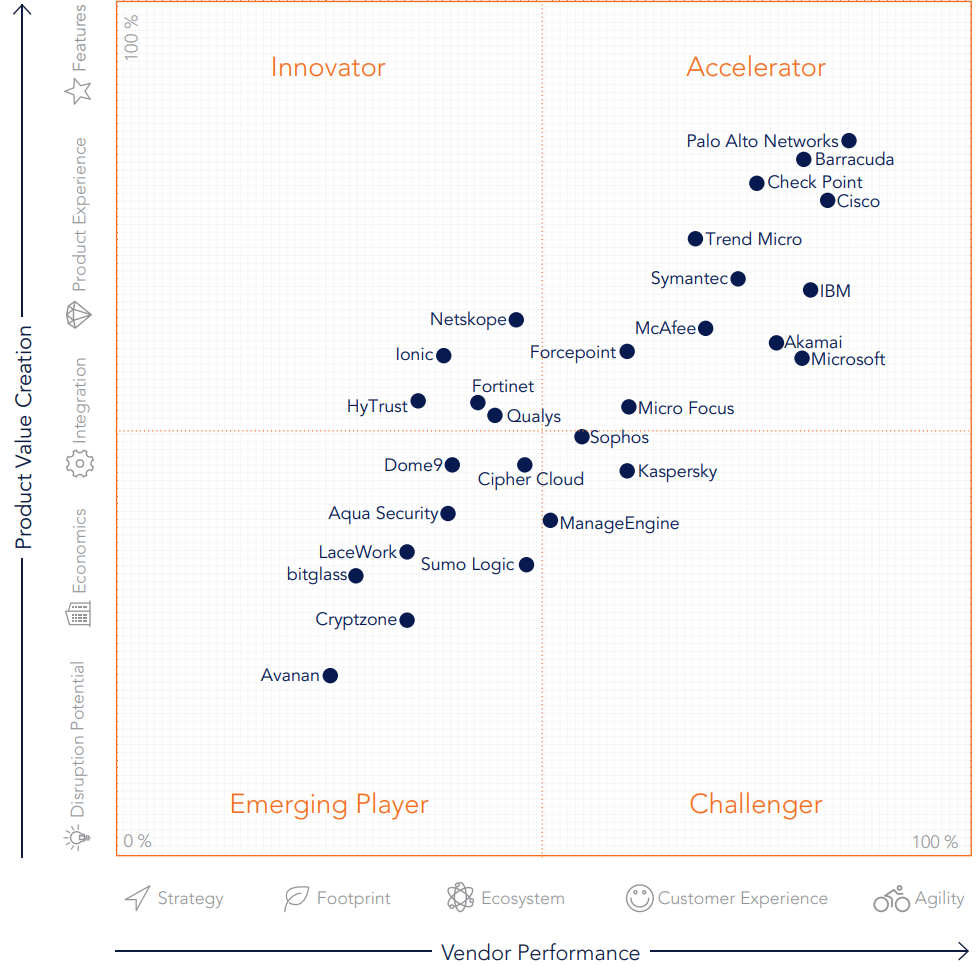
\includegraphics[width=0.8\textwidth]{img/netskopeinnovator.png}
    \caption{Quelle: Crisp Research AG, 2018 - Cloud Security Management Platforms \autocite{Hille2018}}
    \label{fig:netskope}
\end{figure}

\begin{figure}[h]
    \centering
    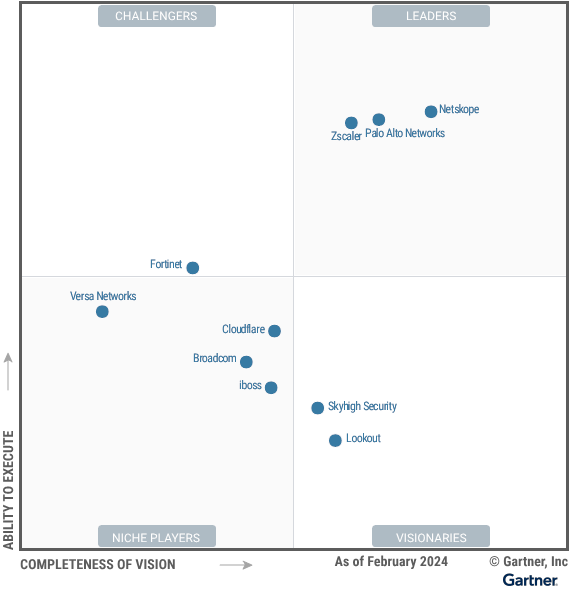
\includegraphics[width=0.8\textwidth]{img/netskope2024.png}
    \caption{Gartner Magic Quadrant voor Security Service Edge (SSE) \autocite{Gartner2024}}
    \label{fig:netskope2024}
\end{figure}


% Netskope onderscheidt zich als een volledig geïntegreerd platform binnen het SASE-framework, met een Secure Service Edge (SSE)-oplossing die DLP, CASB, SWG en ZTNA naadloos combineert. 
% Deze aanpak is waardevol in gedistribueerde werkomgevingen en bij toenemende cloudadoptie \autocite{brouwer2021cloud}. 
% Netskope biedt meer voordelen dan alternatieven zoals Symantec, Digital Guardian, Forcepoint, Microsoft en McAfee. 
% Symantec en Digital Guardian richten zich bijvoorbeeld sterk op endpointbeveiliging, maar missen de cloudfunctionaliteiten die nodig zijn in moderne hybride werkomgevingen. 
% Forcepoint staat bekend om krachtige gedragsanalyses, maar is minder effectief in het ondersteunen van complexe en dynamische cloudomgevingen. 
% Microsoft biedt uitstekende integratie met Office 365, maar hierdoor mist het ook Netskope's cloud-agnostische aanpak, die een breder scala aan cloudapplicaties ondersteunt \autocite{NetskopeTAP2024}. 
% Tenslotte biedt McAfee een breed scala aan beveiligingsoplossingen, maar voor Evolane is Netskope een gebruiksvriendelijker platform met meer flexibiliteit bij het opstellen en aanpassen van regelsets.




% O = onvoldoende
% V = voldoende
% G = goed
% U = uitstekend

% \begin{table}[h]
%     \centering
%     \small
%     \begin{tabular}{p{3cm} p{1.5cm} p{1.5cm} p{1.5cm} p{1.5cm} p{1.5cm} p{1.5cm}}
%         \toprule
%         & \textbf{Cloud-native} & \textbf{SASE/SSE} & \textbf{Flexibele regels} & \textbf{Endpoint focus} & \textbf{SIEM-integratie} & \textbf{Gebruiks\-vriendelijk} \\
%         \midrule
%         Netskope            & U & U & U & U & G & U \\
%         Symantec            & X & X & X & X & G & X \\
%         Microsoft           & X &   &   &   & Vthestral &   \\
%         Forcepoint          & X &   & X & X & G & X \\
%         Digital Guardian    &   &   &   & X &   &   \\
%         McAfee              & X &   & X & X &   &   \\
%         \bottomrule
%     \end{tabular}
%     \caption{Vergelijking van DLP-oplossingen per factor}
%     \label{tab:netskope}
% \end{table}

% Een belangrijke uitdaging bij het implementeren van een Data Loss Prevention (DLP)-oplossing is het omgaan met false positives. 
% Een false positive doet zich voor wanneer een legitieme handeling onterecht als een beveiligingsincident wordt aangeduid. 
% Dit kan leiden tot operationele vertragingen, frustratie bij eindgebruikers en een verlaagde efficiëntie van het systeem. 
% In het geval van Netskope kan een verkeerd geclassificeerd bestand – 
% bijvoorbeeld een legitiem gedeeld rapport dat persoonlijke namen bevat – leiden tot een geblokkeerde workflow of onnodige escalaties.

% Volgens Olateju et al. (2024) vormen false positives een bijzonder knelpunt in AI-gedreven anomaliedetectiesystemen. 
% Hun studie benadrukt hoe een oversensitieve configuratie de nauwkeurigheid verlaagt en tot alertmoeheid leidt bij analisten, 
% wat het risico verhoogt dat echte incidenten over het hoofd worden gezien . 
% Ze stellen tevens dat fine-tuning en continue validatie van modellen essentieel zijn voor het behoud van een werkbare balans tussen veiligheid en gebruiksgemak .

% Ook Lukas (2023) wijst op de uitdagingen van false positives in taalmodellen die worden toegepast in beveiligingscontexten. 
% Zijn onderzoek toont aan dat modellen soms irrelevante of niet-gevoelige informatie als "gevoelig" classificeren, wat leidt tot valse alarmen. 
% Dit is vooral problematisch wanneer DLP-oplossingen gebruik maken van machine learning voor patroonherkenning in natuurlijke taal – 
% iets wat in moderne platforms zoals Netskope steeds vaker het geval is.

% Om deze problematiek te verhelpen, zijn meerdere technieken noodzakelijk:
% Training op domeinspecifieke datasets, zodat modellen context beter begrijpen.
% Gebruik van meerdere detection layers, bijvoorbeeld reguliere expressies in combinatie met ML-gebaseerde detectie.
% Feedback loops, waarin meldingen door gebruikers worden bevestigd of tegengesproken om toekomstige detecties te verbeteren.
% Threshold management, om de gevoeligheid van detectie af te stemmen op bedrijfsbehoeften.
% De balans tussen beveiliging en bruikbaarheid is cruciaal: een te strikte configuratie leidt tot hinder, terwijl een te lakse aanpak risico’s creëert. Netskope biedt hier mogelijkheden tot fijnmazige afstelling, onder andere via confidence levels, policy exceptions en custom DLP rules.
% Kortom, false positives zijn onvermijdelijk in elk geautomatiseerd detectiesysteem, maar door een combinatie van techniek, feedbackmechanismen en zorgvuldig beheer kan hun impact sterk beperkt worden.

% In het onderzoek van Lukas (2023) wordt dieper ingegaan op de problematiek van false positives bij het gebruik van taalmodellen binnen beveiligingscontexten, zoals bij Data Loss Prevention (DLP). Zijn analyse wijst uit dat deze modellen vaak geneigd zijn om ook niet-gevoelige of contextueel irrelevante informatie verkeerd te classificeren als “gevoelig”. Deze overdetectie is problematisch, vooral wanneer modellen op natuurlijke taal getraind zijn en in productieomgevingen zoals Netskope DLP ingezet worden .

% Concreet stelt Lukas dat deze false positives voortkomen uit:
% Overmatige generalisatie van patronen: Het taalmodel associeert bepaalde woordcombinaties (zoals e-mailadressen of namen) automatisch met gevoeligheid, zonder voldoende contextuele verificatie.
% Gebrek aan semantisch onderscheid: De modellen begrijpen onvoldoende het verschil tussen bv. een fictieve naam in een handleiding versus een echte naam in een medisch verslag.
% Bias in trainingsdata: Als de trainingsgegevens oververtegenwoordigd zijn met bepaalde formats of types van informatie, zal het model die patronen als gevoelig beschouwen, ook als dat in de praktijk niet klopt.
% Om deze problematiek te verhelpen, beveelt het onderzoek meerdere technieken aan:
% Context-aware classificatie: In plaats van alleen naar entiteit-types te kijken (zoals "e-mailadres"), moet ook de semantische en syntactische context meewegen.
% Feedback-loops met menselijke evaluatie: Door gebruikers meldingen te laten beoordelen (correct / fout), kan het model bijgestuurd worden.
% Hybride benaderingen: Combinatie van patroon-gebaseerde detectie (regex, heuristieken) en ML om precisie te verhogen.
% Confidence scoring en drempels: Enkel waarschuwingen genereren als het model een hoge mate van zekerheid heeft.

\section{False Positives}
\label{sec:false-positives-literatuurstudie}

False positives bij een DLP-systeem ontstaan wanneer legitieme gegevens onterecht als confidentieel worden geclassificeerd.
Dit kan leiden tot  \textit{\textbf{onnodige waarschuwingen}}, \textit{\textbf{vertragingen in bedrijfsprocessen}} en \textit{\textbf{frustratie bij eindgebruikers}}. 
% Bij overmatige false positives kunnen gebruikers belangrijke waarschuwingen negeren, wat leidt tot \textit{\textbf{alertmoeheid}}.
\textcite{Lukas2023} legt uit dat dit probleem vooral voorkomt in systemen die gebruik maken van machine learning (\gls{ml}) en natuurlijke taalverwerking (\gls{nlp}). 
Dit komt doordat deze systemen vaak niet in staat zijn om de context van gegevens correct te interpreteren, wat leidt tot onjuiste classificaties.
Concreet stelt \textcite{Lukas2023} dat deze false positives vooral voorkomen door:

\begin{itemize}
    \item \textbf{Overmatige generalisatie van patronen}: Het taalmodel associeert bepaalde woordcombinaties, zoals e-mailadressen of namen, automatisch met gevoeligheid, zonder voldoende contextuele verificatie.
    \item \textbf{Gebrek aan semantisch onderscheid}: De modellen begrijpen onvoldoende het verschil tussen bv. een fictieve naam in een handleiding versus een echte naam in een medisch verslag.
   \item \textbf{Bias in trainingsdata}: Als de trainingsgegevens oververtegenwoordigd zijn met bepaalde formats of types van informatie, zal het model die patronen als gevoelig beschouwen, ook als dat in de praktijk niet klopt.
\end{itemize}

\textcite{Olateju2024} stelt vast dat DLP-systemen gemiddeld een false positive-percentage van 4\% tot 5\% vertonen, zelfs bij gebruik van geavanceerde deep learning-algoritmen.
Dit lijkt misschien beperkt, maar in grote organisaties of cloudomgevingen met duizenden datatransacties per dag kan dit resulteren in een aanzienlijke hoeveelheid foutieve waarschuwingen.



% De gevolgen zijn niet louter technisch van aard. 
% False positives leiden tot toegenomen werkdruk voor beveiligingsteams, 
% vertraging van workflows en verminderde gebruikersbetrokkenheid. 
% In het ergste geval ontstaat alertmoeheid, waarbij echte beveiligingsincidenten over het hoofd worden gezien omdat gebruikers of
% analisten gewend raken aan irrelevante meldingen. Dit vergroot het risico op datalekken en non-compliance met wetgeving zoals GDPR of PCI DSS.

% Hoewel volledige eliminatie van false positives onrealistisch is, 
% zijn er diverse manieren om hun impact te beperken. 
% Dit kan via contextuele classificatie, hybride detectiemethoden, 
% en het integreren van gebruikersfeedback in het leerproces van modellen. 
% Moderne platforms zoals Netskope bieden daarnaast concrete instellingen om detectiegevoeligheid te beheren via confidence scores, 
% policy exceptions en maatwerkregels. 
% Door technische, menselijke en beleidsmatige maatregelen te combineren, kan een werkbare balans worden gevonden tussen beveiliging en gebruiksgemak.



% False positives ontstaan wanneer een DLP-systeem onterecht normale gegevens als confidentieel identificeert. 
% Dit kan leiden tot onnodige waarschuwingen en vertragingen in de bedrijfsprocessen.
% Om false positives te vermijden, kan in Netskope bij custom identifiers worden aangegeven dat een bepaald keyword in de buurt moet staan, zoals `RRN' of `Rijksregisternummer'. 
% Hierdoor ziet Netskope het niet als een match of zal het een lagere vertrouwheidsscore geven.
% \autocite{Lukas2023}


% In sectoren zoals de publieke sector en cloud service providers worden grote hoeveelheden gevoelige gegevens verwerkt, w
% aaronder persoonsgegevens (PII) en betalingsgegevens (PCI). 
% Om deze data te beschermen worden Data Leakage Prevention (DLP)-systemen ingezet die gebruikmaken van AI en machine learning om potentieel 
% ongewenste gegevensoverdracht te detecteren. Ondanks technologische vooruitgang kampen deze systemen met een gemiddeld false positive-percentage 
% van circa 4{,}23\%~\cite{detectionaccuracy}. Dit betekent dat een aanzienlijk deel van de gegenereerde waarschuwingen onterecht is, wat verstrekkende
% gevolgen kan hebben voor operationele processen en compliance.

% \subsection{Concreet effect van false positives}
% De aanwezigheid van false positives heeft meerdere negatieve effecten:

% \begin{itemize}
%     \item \textbf{Vertraging van workflows}: Valse meldingen onderbreken bedrijfsprocessen, omdat elke waarschuwing handmatig moet worden gevalideerd. In omgevingen met hoge volumes, zoals overheidsinstanties, leidt dit tot significante vertragingen.
%     \item \textbf{Toegenomen werkdruk}: Security teams worden geconfronteerd met een verhoogde werklast. Onterechte waarschuwingen vergen tijd en middelen die anders besteed zouden worden aan het behandelen van daadwerkelijke incidenten.
%     \item \textbf{Gebruikersfrustratie en verminderde betrouwbaarheid}: Wanneer eindgebruikers regelmatig geconfronteerd worden met valse alarmen, kan dit leiden tot frustratie, verminderde acceptatie van het systeem, en in sommige gevallen zelfs het negeren van belangrijke waarschuwingen (alert fatigue).
%     \item \textbf{Compliance- en veiligheidsrisico's}: Overmatige false positives kunnen ervoor zorgen dat echte datalekken over het hoofd worden gezien. Dit vergroot het risico op non-compliance met regelgeving zoals GDPR of PCI DSS, en kan ernstige gevolgen hebben voor de organisatie.
% \end{itemize}





% Binnen cloudomgevingen en de publieke sector zijn de gevolgen van false positives extra problematisch vanwege de schaal en gevoeligheid van de verwerkte gegevens.
% Hoewel sommige recente studies verbeteringen rapporteren in detectienauwkeurigheid door het gebruik van deep learning 
% (bijv. 3{,}90\% false positives versus 4{,}35\% bij decision trees~\cite{detectionaccuracy}), ligt de focus in de literatuur hoofdzakelijk op technische performance metrics.

% Er is opvallend weinig onderzoek dat zich richt op de operationele impact van deze valse meldingen. 
% Factoren zoals workflowvertraging, menselijke belasting en verminderde gebruikersvertrouwen worden zelden gekwantificeerd, ondanks hun potentiële invloed op de effectiviteit van DLP-systemen.

% \subsection{Onderzoeksnoden en aanbevelingen}

% Deze lacune in de literatuur onderstreept de nood aan meer contextueel onderzoek, met focus op:

% \begin{itemize}
%     \item Het kwantificeren van de operationele impact van false positives in praktijksituaties.
%     \item Het betrekken van eindgebruikers en security professionals in kwalitatieve analyses (zoals casestudies of interviews).
%     \item Het ontwikkelen van verbeterde validatie- en feedbackmechanismen binnen DLP-workflows.
% \end{itemize}
% Toekomstig onderzoek zou de brug moeten slaan tussen technische prestatieverbeteringen en hun reële effect op organisaties. 
% Dit is essentieel om het vertrouwen in DLP-systemen te versterken en de bescherming van PII- en PCI-gegevens in gevoelige sectoren duurzaam te garanderen.




\section{Juridisch kader voor gegevensbescherming in België}%

De bescherming van persoonlijke en bedrijfsinformatie is een essentieel aspect van de hedendaagse digitale samenleving. 
Op zowel nationaal als Europees niveau zijn er wettelijke richtlijnen opgesteld om organisaties te ondersteunen bij het garanderen van de vertrouwelijkheid, 
integriteit en toegankelijkheid van gegevens.

\subsection{Algemene Verordening Gegevens\-besch\-erming (AVG)}%

Dit onderzoek zal in overeenstemming zijn met de Algemene Verordening Gegevensbescherming (AVG of GDPR) 2016/679 van 27 april 2016 \autocite{eu_avg2016} en de Belgische wet van 30 juli 2018 \autocite{BelgischeOverheid2018}.
Volgens de \textcite{eu_avg2016}, overweging (78), moeten passende, technische en organisatorische maatregelen worden genomen om de rechten van natuurlijke personen te beschermen. 
Deze overweging zorgt ervoor dat persoonsgegevens op een veilige en verantwoorde manier worden verwerkt. 
Zo'n beveiliging kan gebeuren door middel van standaardinstellingen die erop zijn gericht om risico's in elke fase van de verwerking van gegevens te minimaliseren.
Op 25 juli 2024 publiceerde de Europese Unie haar tweede verslag over de toepassing van de AVG \autocite{eu_avg2024}. 
Dit rapport legt de nadruk op het feit dat de AVG, ondanks verschillende uitdagingen, een goede basis is voor het veilig en transparant behandelen van persoonsgegevens. 


\subsection{Payment Card Industry Data Security Standard (PCI DSS)}%

De Payment Card Industry Data Security Stand\-ard (\gls{pcidss}) bestaat uit een reeks richtlijnen en regels die ontworpen zijn voor organisaties die betalingsinformatie en kaartinformatie verwerken, 
zoals debit-/ creditcardnummers, Primary Account Numbers (\gls{pan}) en Sensitive Authentication Data (\gls{sad}), zoals Card Verification Value (\gls{cvv}) en magnetische stripgegevens, van alle grote kaartsche\-ma's. 
Deze standaard is ontwikkeld om de veiligheid van kaartinformatie te garanderen en vereist dat organisaties maatregelen nemen om de gegevens van kaarthouders te beschermen \autocite{Elluri2018}. 
\gls{pcidss} vereist de implementatie van toegangscontroles, zoals \gls{dcs}\textbf{-02} (toegangscontrole tot systemen en gegevens), \gls{dcs}\textbf{-07} (beheer van gebruikersidentiteiten en -toegang), 
en \gls{dcs}\textbf{-08} (toegangscontrole tot netwerken en systemen), om de veiligheid van kaartinformatie en de bescherming van kaarthoudergegevens te waarborgen \autocite{Elluri2018}.

\subsection{ISO 27001: Informatiebeveiliging}%

Bovendien moet de DLP-oplossing rekening houden met de vereisten van \gls{iso}, de internationale norm voor het beheer van informatiebeveiliging. 
In dit verband bespreken \textcite{Alsanabani2020} de noodzaak van DLP-oploss\-ingen die zowel detectie- als preventieve methoden samenbrengen. 
De preventieve aanpak probeert datalekken te vermijden door onder andere het gehele confidentiële bestand te versleutelen, toegangscontrole aan te passen en het labelen van de inhoud.

\subsection{Nationale en Europese richtlijnen}%

Buiten de Belgische wetgeving zijn er ook tal van Europese richtlijnen en nationale standaarden die een belangrijke rol hebben in de bescherming van bedrijfsdata. 
Hierbij kan gedacht worden aan de Algemene Verordening Gegevensbescherming (\gls{avg}), de EU Cybersecurity Act en belangrijke Europese richtlijnen, waaronder de \gls{nis2}-richtlijn. 
Deze richtlijnen worden verder uitgebreid met specifieke normen, zoals de \gls{pcidss} voor betalingsgegevens en internationale normen, zoals \gls{iso} voor de beveiliging van informatie. 
De \gls{nis2}-richtlijn (Richtlijn (EU) 2022/2555), die op 16 januari 2023 is aangenomen door de \textcite{nis2directive}, 
heeft als doel de cyberbeveiliging binnen de EU te versterken door een hoog niveau van beveiliging te waarborgen voor netwerken en informatiesystemen. 
Artikel 21 van de \gls{nis2}-richtlijn richt zich op de beveiliging van netwerken en informatiesystemen en legt de verplichting op aan lidstaten om 
ervoor te zorgen dat aanbieders van essentiële en belangrijke diensten passende technische en organisatorische maatregelen nemen. 
Maatregelen die over het DLP-systeem kunnen gaan, zijn onder andere: 

\begin{itemize}
    \item Risicoanalyse (lid 2, punten a en e): Organisaties moeten een risicobeheerproces implementeren dat hen in staat stelt om risico's voor de beveiliging van netwerken en informatiesystemen te identificeren, te evalueren en te beheersen.
    \item Encryptie en toegangscontroles (lid 2, punten h en i): Het gebruik van encryptie, toegangscontroles en regelmatige beveiligingstests en audits.
    \item Incidentenbehandeling (lid 2, punt b): Organisaties moeten procedures en mechanismen hebben voor het detecteren, melden en reageren op beveiligingsincidenten.
    \item Bewustwording en training (lid 2, punt g): Opleidingen om medewerkers te informeren over goede cyberhygiëne en risicomanagement \autocite{nis2directive}. Het DLP-systeem van Netskope staat in voor het trainen van de eindgebruiker, mocht deze iets foutief doen.
\end{itemize}

De studie van \textcite{Nayak2020} geeft een uitgebreid overzicht van systemen voor het detecteren en voorkomen van datalekken, 
inclusief de indeling van systemen op basis van de status van de gegevens (data-at-rest, data-in-motion, dat\-a-in-use) en de detectietechnieken. 
Dit overzicht zal gebruikt worden voor het ontwikkelen van regex-gebaseerde regels in DLP-oploss\-ingen. 
De studie legt de nadruk op het feit dat datalekken zowel onvoorzien als opzettelijk kunnen optreden en geeft uitdagingen aan, 
zoals het identificeren van gevoelige informatie, het balanceren van de detectienauwkeurigheid en de integratie van geavanceerde methodologieën.

% \subsection{Gegevensoverdracht en internationale implicaties}%

\subsection{Andere relevante wetgeving}%

Tabel \ref{tab:wetgeving_dlp} bevat de belangrijkste wettelijke richtlijnen en uitspraken die relevant zijn voor het ontwerp en de implementatie van een Data Leakage Prevention-oplossing voor Belgische bedrijven.

% \begin{figure}
%     \centering
%     % \includegraphics[width=.2\textwidth]
%     \includegraphics[scale=0.50]
%     {img/overzicht.png}
%     \caption{\label{fig:overzicht}Overzicht van de belangrijkste wettelijke richtlijnen en uitspraken voor DLP-oplossingen in België.}
%   \end{figure}

  
  \begin{table}[h]
    \centering
    \small
    \begin{tabular}{p{4cm} p{5cm} p{6cm}}
        \toprule
        \textbf{Wetgeving} & \textbf{Doel} & \textbf{Relevantie voor DLP} \\
        \midrule
        \gls{avg} & Bescherming persoonsgegevens & Dataclassificatie en toegangscontrole \\
        \gls{pcidss} & Beveiliging van betalingsgegevens & Encryptie en toegangsbeheer \\
        \gls{iso} & Informatiebeveiliging & Risicoanalyse en ISMS-implementatie \\
        \gls{ccb}-framework & Strategie voor cybersecurity België & Aanbevelingen voor risicobeheer \\
        \gls{nis2} & Beveiliging netwerken en diensten & Incidentrapportage en risicoanalyse \\
        EU Cybersecurity Act & Certificering van beveiligingstechnologie & DLP-oplossingen certificeren \\
        Schrems II & Gegevensoverdracht naar niet-EU-landen & Beperking van cloud-gebaseerde opslag \\
        \bottomrule
    \end{tabular}
    \caption{Overzicht van wetgeving en relevantie voor DLP}
    \label{tab:wetgeving_dlp}
\end{table}


  

\section{Ethische overwegingen}%

Een essentieel aspect van de implementatie van DLP is het vinden van de juiste balans tussen gegevensbeveiliging en gebruikersprivacy. 
Het gebruik van DLP-systemen kan leiden tot het monitoren van gebruikersgedrag, wat kan worden gezien als een inbreuk op de privacy van medewerkers. 
Om het vertrouwen bij medewerkers en klanten te behouden, is het belangrijk om transparant te zijn over het gebruik van DLP-systemen en de redenen daarvoor. 
Hierdoor weet elke gebruiker welke gegevens worden verzameld en hoe deze worden gebruikt \autocite{Zaini2024}. 
Deze regelsets moeten niet alleen voldoen aan de wettelijke vereisten, maar ook aan de ethische normen en waarden van de organisatie. 
Om monitoring van data en gebruikersgedrag te minimaliseren, 
zal de implementatie van de DLP-oplossing specifiek gericht zijn op het beschermen van gevoelige gegevens en het voorkomen van datalekken. 

Tijdens het vak \textit{IT Professional \& Career Orientation (ITPCO)} kwam het belang van ethische en juridische aspecten binnen informatieveiligheid uitgebreid aan bod. 
Gastspreker \textcite{SoficoGuestLecture2024} van \textit{Sofico} presenteerde een overzicht van hoe een internationaal bedrijf dat softwareoplossingen ontwikkelt voor autofinanciering, 
leasing, fleetmanagement en mobiliteitsbeheer, privacy en compliance structureel integreert in zijn processen \autocite{SoficoGuestLecture2024}. 
Het gastcollege behandelde onder meer fysieke beveiligingsmaatregelen, toegangsbeheer tot ontwikkelomgevingen en de inzet van white hat hackers voor het identificeren van kwetsbaarheden.
De organisatie gebruikt principes zoals \textit{Privacy by Design} en \textit{Security by Design} binnen de volledige ontwikkeling en implementatie van software. 
Deze principes staan in lijn met de \gls{avg} en \gls{iso} normen, waarbij de focus ligt op het minimaliseren van gegevensverwerking en het behouden van de privacy van gebruikers.
De inzichten van Sofico zijn rechtstreeks van toepassing op dit onderzoek.
\textit{Privacy by Design} en \textit{Security by Design} zijn namelijk gericht op minimale gegevensverwerking, transparantie, logging en traceerbaarheid. 
Binnen \textcite{Netskope2024PrivByDesign} worden deze principes toegepast via \textit{\textbf{in-memory verwerking}}, \textit{\textbf{gegevensobfuscatie}}, \textit{\textbf{klantgecontroleerde datalokalisatie}} en \textit{\textbf{uitgebreide transactie-logging}}.

% Tijdens het vak \textit{IT Professional \& Career Orientation (ITPCO)} werd aandacht besteed aan de ethische, 
% juridische en organisatorische aspecten van gegevensverwerking en informatieveiligheid. 
% Deze inzichten zijn rechtstreeks van toepassing op dit onderzoek, 
% dat zich toespitst op de implementatie van een DLP-oplossing binnen een cloud- en compliancegevoelige omgeving.

% Een bijzonder waardevol onderdeel van het vak was het gastcollege door een medewerker van Sofico, 
% een internationaal softwarebedrijf actief binnen de automotive-sector. 
% Dit college illustreerde hoe bedrijven zoals Sofico concreet omgaan met databeveiliging, 
% toegangsbeheer en regelgeving zoals de AVG en ISO/IEC 27001. De spreker benadrukte onder andere het belang van:

% \begin{itemize}
%   \item \textbf{Data Classification en Secure Development:} het correct classificeren en beveiligen van data over de volledige softwareontwikkelingscyclus, conform het principe van \textit{Privacy by Design}.
%   \item \textbf{Datalekken en verantwoordelijkheden:} een datalek moet binnen 24 uur gemeld worden aan de bevoegde autoriteiten (zoals de GBA in België). Hiervoor zijn rollen zoals de \textit{Data Protection Officer (DPO)} essentieel.
%   \item \textbf{\gls{iso}-certificatie:} organisaties worden via deze norm verplicht om informatieveiligheid systematisch aan te pakken. Topics zoals thuiswerken, wachtwoordbeheer, netwerkstructuren en leveranciersbeheer worden hierbij geëvalueerd.
% \end{itemize}

% Deze inzichten waren bijzonder relevant gezien mijn bachelorproef een DLP-oplossing onderzoekt die PII/PCI-gegevens in de cloud moet beschermen. 
% Vanuit ethisch oogpunt is het cruciaal om dataminimalisatie, transparantie en toestemming (\textit{lawfulness, fairness, transparency}) 
% centraal te plaatsen in zowel ontwerp als configuratie. 
% Daarnaast vormde het college een reflectiemoment: in welke mate houdt mijn stagebedrijf zelf rekening met deze normen en 
% is het bewust van certificeringsvereisten zoals ISO/IEC 27001?

%%=============================================================================
%% Methodologie
%%=============================================================================

\chapter{\IfLanguageName{dutch}{Methodologie}{Methodology}}%
\label{ch:methodologie}

%% TODO: In dit hoofstuk geef je een korte toelichting over hoe je te werk bent
%% gegaan. Verdeel je onderzoek in grote fasen, en licht in elke fase toe wat
%% de doelstelling was, welke deliverables daar uit gekomen zijn, en welke
%% onderzoeksmethoden je daarbij toegepast hebt. Verantwoord waarom je
%% op deze manier te werk gegaan bent.
%% 
%% Voorbeelden van zulke fasen zijn: literatuurstudie, opstellen van een
%% requirements-analyse, opstellen long-list (bij vergelijkende studie),
%% selectie van geschikte tools (bij vergelijkende studie, "short-list"),
%% opzetten testopstelling/PoC, uitvoeren testen en verzamelen
%% van resultaten, analyse van resultaten, ...
%%
%% !!!!! LET OP !!!!!
%%
%% Het is uitdrukkelijk NIET de bedoeling dat je het grootste deel van de corpus
%% van je bachelorproef in dit hoofstuk verwerkt! Dit hoofdstuk is eerder een
%% kort overzicht van je plan van aanpak.
%%
%% Maak voor elke fase (behalve het literatuuronderzoek) een NIEUW HOOFDSTUK aan
%% en geef het een gepaste titel.
%% \lipsum[21-25]

Het onderzoek naar de ontwikkeling en integratie van een Netskope-gebaseerde Data Leakage Prevention (DLP)-oplossing binnen 
de bedrijfsomgeving van Evolane. De onderzoeksmethode is een combinatie van een literatuurstudie en een praktische Proof of Concept (PoC).

\section{Literatuurstudie}%

Het onderzoek begint met een uitgebreide literatuurstudie naar bestaande DLP-oplossingen, Netskope's Secure Service Edge (\gls{sse}) platform en de relevante Belgische en Europese wetgevingen. 
Hierbij wordt gebruik gemaakt van academische artikelen, technische documentatie en juridische bronnen om een basis te leggen. 
Voor de literatuurstudie is ongeveer twee weken voorzien, waarin de focus ligt op het verder verzamelen en verwerken van recente bronnen
over DLP-technologie, juridische eisen (\gls{avg}, \gls{pcidss}, \gls{nis2}) en Netskope's DLP-oplossing.

\section{Analyse en planning}%

Na de literatuurstudie volgt de selectie van specifieke datasets, zoals persoonlijk identificeerbare informatie (\gls{pii}) en betalingsgegevens (\gls{pci}), voor testen binnen de PoC.
Een voorbeeld hiervan zijn de synthetische e-maildatasets van \textcite{Whelan2014}. 
Deze datasets bevatten in totaal 4796 e-mails, waarvan 4010 geen \gls{pii} bevatten en 786 e-mails dit wel hebben, 
waaronder adressen, creditcardnummers en namen. 
De opgestelde testscenario's sluiten aan bij de bedrijfsprocessen van Evolane, zoals e-mailverkeer en bestandsoverdrachten naar cloudservices. 
Naast deze scenario's richt de analyse zich ook op de workflow van eindgebruikers, met als doel False Positives te beperken en de de workflow van de eindgebruikers niet te verstoren.
Deze fase begint al deels tijdens de literatuurstudie en duurt ongeveer drie weken.

\section{Risicoanalyse}%

Een belangrijk onderdeel van dit onderzoek is het uitvoeren van een risicoanalyse, waarbij mogelijke technische, juridische en organisatorische risico's worden geïdentificeerd en beoordeeld. 
Technische risico's kunnen bijvoorbeeld bestaan uit het niet volledig detecteren van gevoelige gegevens of prestatieproblemen van het DLP-systeem. 
Juridische risico's hebben te maken met het niet naleven van de \gls{avg}-vereisten of andere relevante wetgeving. 
Organisatorische risico's omvatten mogelijke weerstand van medewerkers tegen nie\-uwe beveiligingsmaatregelen of een gebrek aan training, 
wat de effectiviteit van de DLP-oplossing kan verminderen. 
Voor elk vastgesteld risico worden geschikte maatregelen genomen om de gevolgen te beperken. 
Deze fase duurt ongeveer twee weken, overlappend met Analyse en Planning. Op het vlak van expertise zal hierbij de co-promotor van Evolane betrokken worden. 

\subsection{Technische risico's}

Technische risico's zijn gerelateerd aan de operationele elementen van de DLP-oplossing en de technische infrastructuur van Evolane.
Een van de belangrijkste technische risico's is de onvolledige detectie van confidentiële gegevens. 
Het DLP-systeem kan mogelijk niet alle vormen van \gls{pii} en \gls{pci} detecteren, vooral als er nieuwe of onbekende datatypes worden gebruikt.
Daarnaast kan de implementatie van Netskope leiden tot prestatieproblemen, zoals vertragingen in netwerkverkeer of een verhoogd gebruik van systeemresources.
Integratieproblemen vormen een ander potentieel risico, aangezien het DLP-systeem moet werken met bestaande IT-infrastructuren.
Onverwachte compatibiliteitsproblemen kunnen de implementatie vertragen. Vervolgens kunnen verdere beveiligingslekken ontstaan 
door onvoldoende configuratie of zwakke punten in het DLP-systeem, waardoor confidentiële data alsnog kan worden gelekt.
Om deze technische risico's te mitigeren, zullen uitgebreide tests worden uitgevoerd om de detectienauwkeurigheid van het DLP-systeem te waarborgen.
Daarnaast zullen systeemprestaties worden gemonitord tijdens de implementatie en indien nodig optimalisaties worden doorgevoerd om prestatieproblemen te minimaliseren.
Tenslotte zal een plan worden opgesteld hoe het DLP-systeem veilig geüpdatet kan worden om potentiële kwetsbaarheden te vermijden.

\subsection{Juridische risico's}

Juridische risico's hebben betrekking op de naleving van wet- en regelgeving, zoals de Algemene Verordening Gegevensbescherming (\gls{avg}) en de NIS2-richtlijn.
Onvoldoende naleving van deze wetten en richtlijnen (waaronder \gls{avg}, \gls{pci} DSS, ISO 27001, NIS2, Schrems II,..) kan leiden tot juridische sancties. 
Een belangrijk juridisch risico betreft onjuiste Data Processing Agreements (\gls{dpa}) met dataverwerkers. 
Verkeerde of ontbrekende overeenkomsten met dataverwerkers kunnen juridische complicaties veroorzaken. 
Daarnaast kan het niet correct toepassen van dataminimalisatieprincipes of het verwerken van data voor andere doeleinden dan waarvoor ze zijn verzameld, 
ook leiden tot juridische gevolgen. 
Om deze juridische risico's te beperken, stellen betrokken partijen zorgvuldig \gls{dpa}'s op en voeren zij regelmatige herzieningen uit.

\subsection{Organisatorische risico's}

Organisatorische risico's hebben betrekking op de interne processen en procedures van Evolane en de acceptatie van de DLP-oplossing door medewerkers. 
Weerstand van medewerkers kan een belangrijk organisatorisch risico vormen, aangezien medewerkers mogelijk niet openstaan voor nieuwe beveiligingsmaatregelen. 
Een gebrek aan training kan bovendien leiden tot misbruik of onjuist gebruik van het DLP-systeem, wat de effectiviteit ervan zal verminderen. 
Om dan tenslotte deze organisatorische risico's te mitigeren, zullen workshops en informatiesessies worden georganiseerd om medewerkers te betrekken en het belang van de DLP-oplossing te benadrukken. 
Door medewerkers actief te betrekken en voldoende training te bieden, wordt het gebruik van de DLP-oplossing vergroot en wordt de effectiviteit ervan versterkt.

\section{Proof of Concept}%

De PoC wordt opgezet in een interne testomgeving binnen het bedrijf, waarbij een Netskope-licentie wordt gebruikt om de DLP-service in te stellen. 
Deze omgeving zal verschillende datatypes bevatten (data-in-use, data-in-motion, data-at-rest), 
waarbij zowel vertrouwelijke als niet\--vertr\-ouwelijke bestanden worden gebruikt om te testen of de DLP-service alle vertrouwelijke data effectief kan identificeren en verdere verwerking kan blokkeren. 
De data bestaat voornamelijk uit persoonlijk identificeerbare informatie (\gls{pii}) en betalingsgegevens (\gls{pci}), die volgens de geldende wet- en regelgeving (zoals \gls{avg}, \gls{pci} DSS, ISO 27001, NIS2, Schrems II, enz.) beschermd moeten worden. 
Gebruikers met verschillende rechten zullen data doorsturen en verwerken binnen de testomgeving. 
De duur van de PoC is afhankelijk van de complexiteit van de testscenario's en de detectie van gevoelige gegevens, 
maar wordt geschat op 5 tot 6 weken. 
Na ongeveer 5 weken zou een eerste evaluatie van de effectiviteit van de DLP-oplossing mogelijk moeten zijn, 
en kan deze aan de eindgebruikers van Evolane worden gepresenteerd. 
Voor de technische uitvoering is expertise nodig in de configuratie van Netskope (bijvoorbeeld het instellen van detectie- en preventieregels met regex-patronen), 
evenals basiskennis van de netwerkinfrastructuur van de testomgeving om de dataflows goed na te bootsen.

\section{Gebruikerstests en feedback}%

Na de initiële implementatie van de PoC worden gebruikers van Evolane betrokken bij het testen van de DLP-oplossing. 
Dit gebeurt, samen met mijn co-promotor, door middel van workshops en praktische tests waarbij eindgebruikers realistische scenario's simuleren waarin gevoelige data verwerkt en verplaatst wordt. 
De feedback van deze gebruikers is essentieel om inzicht te krijgen in de gebruiksvriendelijkheid en de invloed van de DLP-regelsets op de dagelijkse taken. 

\section{Evaluatie en meetbare criteria}%

De effectiviteit van de geïmplementeerde DLP-oplossing wordt geëvalueerd aan de hand van vooraf gedefinieerde Key Performance Indicators (\gls{kpi}'s). 
Deze \gls{kpi}'s dienen als indicator om te beoordelen in hoeverre de DLP-oplossing voldoet aan de gestelde vereisten en doelstellingen.
Detectienauwkeurigheid meet het percentage correct geïdentificeerde confidentiële gegevens binnen de totale dataset, 
wat aangeeft hoe effectief de DLP-oplossing is in het herkennen van \gls{pii} en \gls{pci}. 
Het aantal false positives geeft aan hoeveel gegevens onterecht zijn geblokkeerd of gemarkeerd, 
wat inzicht geeft in de nauwkeurigheid van de detectiemethoden en helpt bij het finetunen van de regelsets. 
Dit zal in een Confusion Matrix worden weergegeven \autocite{Microsoftn.d.}.
Systeemimpact zal het effect van de DLP-implementatie op de algehele systeemprestaties beoordelen, zoals CPU- en 
geheugenverbruik, zodat de oplossing geen significante vertragingen of resource-uitputting zou veroorzaken.

\section{Documentatie van resultaten}%

Alle bevindingen en conclusies worden grondig gedocumenteerd. 
In ongeveer twee weken tijd worden handleidingen, een schriftelijk evaluatierapport en het finale concept-bachelorproef geschreven.

\section{Planning}%
\label{sec:planning}

De planning van het onderzoek, weergegeven in figuur \ref{fig:gantBP}, is vastgelegd in een Gantt-diagram. De planning is opgesteld van 17 februari 2025 tot 24 mei 2025, met de laatste twee weken specifiek gereserveerd voor documentatie.

\begin{figure}
  \centering
  % \includegraphics[width=.2\textwidth]
  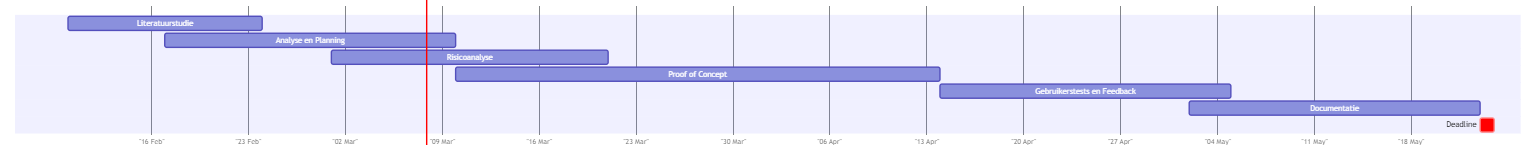
\includegraphics[scale=0.50]
  {img/ganttupdate.png}
  \caption{\label{fig:gantBP}Gantt-diagram van de onderzoeksplanning van 10 februari 2025 tot 23 mei 2025.}
\end{figure}


% Voeg hier je eigen hoofdstukken toe die de ``corpus'' van je bachelorproef
% vormen. De structuur en titels hangen af van je eigen onderzoek. Je kan bv.
% elke fase in je onderzoek in een apart hoofdstuk bespreken.

%\input{...}
%\input{...}
%...

%%=============================================================================
%% Conclusie
%%=============================================================================

\chapter{\IfLanguageName{dutch}{Conclusie}{Conclusion}}%
\label{ch:conclusie}

% TODO: Trek een duidelijke conclusie, in de vorm van een antwoord op de
% onderzoeksvra(a)g(en). Wat was jouw bijdrage aan het onderzoeksdomein en
% hoe biedt dit meerwaarde aan het vakgebied/doelgroep? 
% Reflecteer kritisch over het resultaat. In Engelse teksten wordt deze sectie
% ``Discussion'' genoemd. Had je deze uitkomst verwacht? Zijn er zaken die nog
% niet duidelijk zijn?
% Heeft het onderzoek geleid tot nieuwe vragen die uitnodigen tot verder 
%onderzoek?

% \lipsum[76-80]



%---------- Bijlagen -----------------------------------------------------------

\appendix

\chapter{Onderzoeksvoorstel}

Het onderwerp van deze bachelorproef is gebaseerd op een onderzoeksvoorstel dat vooraf werd beoordeeld door de promotor. Dat voorstel is opgenomen in deze bijlage.

%% TODO: 
%\section*{Samenvatting}

% Kopieer en plak hier de samenvatting (abstract) van je onderzoeksvoorstel.

% Verwijzing naar het bestand met de inhoud van het onderzoeksvoorstel
%---------- Inleiding ---------------------------------------------------------

% TODO: Is dit voorstel gebaseerd op een paper van Research Methods die je
% vorig jaar hebt ingediend? Heb je daarbij eventueel samengewerkt met een
% andere student?
% Zo ja, haal dan de tekst hieronder uit commentaar en pas aan.

%\paragraph{Opmerking}

% Dit voorstel is gebaseerd op het onderzoeksvoorstel dat werd geschreven in het
% kader van het vak Research Methods dat ik (vorig/dit) academiejaar heb
% uitgewerkt (met medesturent VOORNAAM NAAM als mede-auteur).
% 

\section{Inleiding}%
\label{sec:inleiding}

In dit onderzoek wordt een klantenomgeving ontwikkeld voor Evolane, waarin klantengegevens worden verwerkt en opgeslagen. Deze omgeving zal vertrouwelijke gegevens bevatten die beschermd moeten zijn tegen ongeautoriseerde toegang en datalekken. Data Leakage Prevention (DLP) biedt organisaties de mogelijkheid om hun vertrouwelijke informatie te beschermen tegen datalekken en ongeautoriseerde toegang. Het implementeren van een passende DLP-oplossing moet voldoen aan wettelijke vereisten. In België zijn de bekendste de Algemene verordening gegevensbescherming (AVG) en Payment Card Industry Data Security Standards (PCI DSS) voor betalingsgegevens. Ook de NIS2-richtlijnen en cybersecurity-frameworks zoals het CCB-framework of ISO 27001 kunnen  toegepast worden.
De vraag die centraal staat in dit onderzoek is: “Hoe kan een Netskope-gebaseerde DLP-oplossing ontworpen en geïmplementeerd worden om vertrouwelijke gegevens te beschermen en te voldoen aan de Belgische regelgeving?”. Uit deze hoofdvraag kunnen we een aantal deelvragen afleiden:

\begin{itemize}
    \item Welke mogelijkheden biedt Netskope's Secure Service Edge (SSE) platform voor Data Leakage Prevention (DLP) in de context van vertrouwelijke gegevensbescherming?
    \item Hoe kunnen regelsets en dataclassificatie in Netskope DLP worden afgestemd op de Belgische wetgeving, zoals de AVG en NIS2-richtlijn?
    \item Welke technieken en methoden kunnen worden toegepast om persoonsgegevens (PII) en betalingsgegevens (PCI) effectief te detecteren en te beschermen binnen het Netskope-platform?
    \item Hoe kan een Proof of Concept (PoC) voor Netskope DLP worden opgezet in een testomgeving om de effectiviteit van de oplossing te evalueren?
    \item Welke juridische en technische normen moeten worden meegenomen bij het ontwerpen van een DLP-oplossing voor een Belgische organisatie, en hoe kan Netskope aan deze eisen voldoen?
\end{itemize}

% Waarover zal je bachelorproef gaan? Introduceer het thema en zorg dat volgende zaken zeker duidelijk aanwezig zijn:

% \begin{itemize}
%   \item kaderen thema
%   \item de doelgroep
%   \item de probleemstelling en (centrale) onderzoeksvraag
%   \item de onderzoeksdoelstelling
% \end{itemize}

% Denk er aan: een typische bachelorproef is \textit{toegepast onderzoek}, wat betekent dat je start vanuit een concrete probleemsituatie in bedrijfscontext, een \textbf{casus}. Het is belangrijk om je onderwerp goed af te bakenen: je gaat voor die \textit{ene specifieke probleemsituatie} op zoek naar een goede oplossing, op basis van de huidige kennis in het vakgebied.

% De doelgroep moet ook concreet en duidelijk zijn, dus geen algemene of vaag gedefinieerde groepen zoals \emph{bedrijven}, \emph{developers}, \emph{Vlamingen}, enz. Je richt je in elk geval op it-professionals, een bachelorproef is geen populariserende tekst. Eén specifiek bedrijf (die te maken hebben met een concrete probleemsituatie) is dus beter dan \emph{bedrijven} in het algemeen.

% Formuleer duidelijk de onderzoeksvraag! De begeleiders lezen nog steeds te veel voorstellen waarin we geen onderzoeksvraag terugvinden.

% Schrijf ook iets over de doelstelling. Wat zie je als het concrete eindresultaat van je onderzoek, naast de uitgeschreven scriptie? Is het een proof-of-concept, een rapport met aanbevelingen, \ldots Met welk eindresultaat kan je je bachelorproef als een succes beschouwen?

%---------- Stand van zaken ---------------------------------------------------

\section{Literatuurstudie}%
\label{sec:literatuurstudie}

\subsection{Data Leakage Prevention (DLP)}%

Een DLP-systeem heeft als doel drie soorten gegevens binnen een organisatie te beschermen: data-at-rest, data-in-motion en data-in-use. Data-at-rest verwijst naar statische informatie die is opgeslagen in bedrijfssystemen, zoals documentbeheersystemen, e-mailservers, bestandsservers, netwerkschijven, persoonlijke computers en opslagruimtenetwerken (SANs). Data-in-motion verwijst naar bedrijfsinformatie die zich beweegt binnen het uitgaande netwerkverkeer, zoals e-mails en online verkeer. Data-in-use bestaat uit informatie die medewerkers gebruiken op eindgebruikersapparaten, zoals een bestand kopiëren naar een USB-schijf. De definitie van vertrouwelijkheid binnen een organisatie vraagt om een grondigere analyse. Bepaalde soorten informatie, zoals Persoonlijk Identificeerbare Informatie (PII), waaronder namen, identiteitskaart- en creditcardgegevens, behoren in elke organisatie als vertrouwelijk te worden beschouwd. Deze definitie krijgt echter ingewikkeldere aspecten bij bedrijfsgeheimen en interne communicatie, die vaak onregelmatig zijn. Vertrouwelijke informatie verwijst naar gegevens die binnen de organisatie zijn verzameld en niet algemeen toegankelijk zijn. Een DLP-systeem bevat de mogelijkheid om gevoelige gegevens te herkennen in een of meerdere van de genoemde datatypen.


\subsubsection{PCI en PII}
.
\subsubsection{Gegevensverlies detectie methoden}

Identificatiemiddelen worden gebruikt om gevoelige informatie, zoals PII en PCI, te detecteren. Dit gebeurt op basis van reguliere expressies (regex). Regex is een krachtig hulpmiddel dat DLP helpt specifieke gegevenstypen te herkennen door middel van uitdrukkingen, termen en patronen, zoals \texttt{BE\textbackslash d\{2\}\textbackslash s?\textbackslash d\{4\}\textbackslash s?\textbackslash d\{4\}\textbackslash s?\textbackslash d\{4\}} dat kan dienen voor Belgische IBAN-codes. Hoewel dit patroon effectief is voor standaard IBAN-formaten, kan het worden omzeild door een karakter toe te voegen in de invoer, wat de nood benadrukt van extra controles. 

De aangemaakte identificatie voor confidentiële gegevens moet voldoen aan de volgende richtlijnen:

\begin{itemize}
    \item Vooraf gedefinieerde en aanpasbare patronen voor datadetectie: Het is cruciaal om duizenden vooraf ingestelde regels voor het herkennen van gegevens beschikbaar te hebben en deze te kunnen aanpassen aan de behoeften van de organisatie.
    \item Ondersteuning voor verschillende soorten bestandstypen (Word, Excel, PDF, JPG, PNG, CSV, ZIP en RAR, etc.) en categorieën (afbeeldingen, databases, spreadsheets, etc.).
    \item Ondersteuning voor landspecifieke identificatienummers (IBAN's, postcodes, adressen, nationale identiteitskaarten, IP-adressen, paspoort- en telefoonnummers).
    \item Voldoen aan de wet- en regelgeving.
\end{itemize}

De bescherming van PII en PCI-gegevens vormt een kernaspect van DLP. \textcite{Wason2020CASB} legt de nadruk op het belang van de integratie van Cloud Access Security Brokers (CASB) in cloudomgevingen. CASB biedt organisaties de mogelijkheid om een uitgebreide zichtbaarheid te krijgen in het gebruik van cloudtoepassingen, inclusief goedgekeurde en ongeautoriseerde (shadow IT) diensten. Dit helpt enorm bij het identificeren van waar gevoelige gegevens zich bevinden en hoe ze worden verwerkt.

\subsection{Netskope}%

Netskope heeft zich ontwikkeld tot een vooraanstaande speler in cloudbeveiliging door zijn geavanceerde Secure Service Edge (SSE)-platform. Het levert geïntegreerde CASB- en DLP-mogelijkheden. Volgens \textcite{Riley2018} onderscheidt Netskope zich met functies zoals flexibele regelconfiguraties en realtime-detectie van gevoelige data. \textcite{VanDerWalt2022} identificeren belangrijke aspecten binnen Secure Access Service Edge (SASE) frameworks die nog onvoldoende onderzoek bevatten. Dit combineert netwerk- en beveiligingsdiensten in een cloudgebaseerde omgeving. Deze aspecten zijn onder andere de integratie van verschillende beveiligingscomponenten zoals Secure Web Gateways (SWG), CASB en Zero Trust Network Access (ZTNA). Deze onderdelen dienen samen te werken om een integrale beveiligingsstrategie te creëren. Bovendien is er een toenemende vraag naar het ontwikkelen van API-integraties voor Security Information and Event Management (SIEM)-systemen, zodat gegevens uit verschillende bronnen effectief kunnen worden verzameld en geanalyseerd.
\subsection{Juridisch Kader voor Gegevensbescherming in België}%

De bescherming van persoonlijke en bedrijfsinformatie is een essentieel aspect van de hedendaagse digitale samenleving. Op zowel nationaal als Europees niveau zijn er wettelijke richtlijnen opgesteld om organisaties te ondersteunen bij het garanderen van de vertrouwelijkheid, integriteit en toegankelijkheid van gegevens.

\subsubsection{Algemene Verordening Gegevensbescherming (AVG)}%

Dit onderzoek zal in overeenstemming zijn met de Algemene Verordening Gegevensbescherming (AVG of GDPR) 2016/679 van 27 april 2016 \autocite{eu_avg2016} en de Belgische wet van 30 juli 2018 \autocite{wet_bescherming_2018}.
Volgens de \textcite{eu_avg2016}, overweging (78), moeten passende, technische en organisatorische maatregelen worden genomen om de rechten van natuurlijke personen te beschermen. Deze overweging zorgt ervoor dat persoonsgegevens op een veilige en verantwoorde manier worden verwerkt. Zo'n beveiliging kan gebeuren door middel van standaardinstellingen die erop zijn gericht om risico's in elke fase van de verwerking van gegevens te minimaliseren.
Op 25 juli 2024 publiceerde de Europese Unie haar tweede verslag over de toepassing van de AVG \autocite{eu_avg2024}. Dit rapport legt de nadruk op het feit dat de AVG, ondanks verschillende uitdagingen, een goede basis is voor het veilig en transparant behandelen van persoonsgegevens. 


\subsubsection{Payment Card Industry Data Security Standard (PCI DSS)}%

De Payment Card Industry Data Security Standard (PCI DSS) bestaat uit een reeks richtlijnen en regels die ontworpen zijn voor organisaties die betalingsinformatie en kaartinformatie verwerken, zoals debit-/creditcardnummers, Primary Account Numbers (PAN) en Sensitive Authentication Data (SAD) zoals Card Verification Value (CVV) en magnetische stripgegevens, van alle grote kaartschema’s. Deze standaard is ontwikkeld om de veiligheid van kaartinformatie te garanderen en vereist dat organisaties maatregelen nemen om de gegevens van kaarthouders te beschermen \autocite{Elluri2018}. PCI DSS vereist de implementatie van toegangscontroles, zoals DCS-02 (toegangscontrole tot systemen en gegevens), DCS-07 (beheer van gebruikersidentiteiten en -toegang), en DCS-08 (toegangscontrole tot netwerken en systemen), om de veiligheid van kaartinformatie en de bescherming van kaarthoudergegevens te waarborgen \autocite{Elluri2018}.

\subsubsection{ISO 27001: Informatiebeveiliging}%

Bovendien moet de DLP-oplossing rekening houden met de vereisten van ISO 27001, de internationale norm voor het beheer van informatiebeveiliging. In dit verband bespreken \textcite{Alsanabani2020} de noodzaak van DLP-oplossingen die zowel detectie- als preventieve methoden samenbrengen. De preventieve aanpak probeert datalekken te vermijden door onder andere het gehele confidentiële bestand te versleutelen, toegangscontrole aan te passen en het labelen van de inhoud.

\subsubsection{Nationale en Europese Richtlijnen}%

Buiten de Belgische wetgeving zijn er ook tal van Europese richtlijnen en nationale standaarden die een belangrijke rol hebben in de bescherming van bedrijfsdata. Hierbij kan gedacht worden aan de Algemene Verordening Gegevensbescherming (AVG), de EU Cybersecurity Act en belangrijke Europese richtlijnen, waaronder de NIS2-richtlijn. Deze richtlijnen worden verder uitgebreid met specifieke normen, zoals de PCI DSS voor betalingsgegevens en internationale normen, zoals ISO 27001 voor de beveiliging van informatie. 
De NIS2-richtlijn (Richtlijn (EU) 2022/2555), die op 16 januari 2023 is aangenomen door de \cite{nis2directive}, heeft als doel de cyberbeveiliging binnen de EU te versterken door een hoog niveau van beveiliging te waarborgen voor netwerken en informatiesystemen. Artikel 21 van de NIS2-richtlijn richt zich op de beveiliging van netwerken en informatiesystemen en legt de verplichting op aan lidstaten om ervoor te zorgen dat aanbieders van essentiële en belangrijke diensten passende technische en organisatorische maatregelen nemen. maatregelen die over het DLP-systeem kunnen gaan, zijn onder andere: 

\begin{itemize}
    \item Risicoanalyse (lid 2, punten a en e): Organisaties moeten een risicobeheerproces implementeren dat hen in staat stelt om risico's voor de beveiliging van netwerken en informatiesystemen te identificeren, te evalueren en te beheersen.
    \item Encryptie en toegangscontroles (lid 2, punten h en i): Het gebruik van encryptie, toegangscontroles en regelmatige beveiligingstests en audits.
    \item Incidentenbehandeling (lid 2, punt b): Organisaties moeten procedures en mechanismen hebben voor het detecteren, melden en reageren op beveiligingsincidenten.
    \item Bewustwording en training (lid 2, punt g): Opleidingen en bewustwordingsprogramma's om medewerkers te informeren over goede cyberhygiëne en risicomanagement. \autocite{nis2directive} Het DLP-systeem van Netskope staat in voor het trainen van de eindgebruiker, mocht deze iets foutief doen.
\end{itemize}

De studie van \textcite{Nayak2020} geeft een uitgebreid overzicht van systemen voor het detecteren en voorkomen van datalekken, inclusief de indeling van systemen op basis van de status van de gegevens (data-at-rest, data-in-motion, data-in-use) en de detectietechnieken. Dit overzicht zal gebruikt worden voor het ontwikkelen van regex-gebaseerde regels in DLP-oplossingen. De studie legt de nadruk op het feit dat datalekken zowel onvoorzien als opzettelijk kunnen optreden en geeft uitdagingen aan, zoals het identificeren van gevoelige informatie, het balanceren van de detectienauwkeurigheid en de integratie van geavanceerde methodologieën.

% \subsubsection{Gegevensoverdracht en internationale implicaties}%

\subsubsection{Andere relevante wetgeving}%

De onderstaande tabel bevat de belangrijkste wettelijke richtlijnen en uitspraken die relevant zijn voor het ontwerp en de implementatie van een Data Leakage Prevention-oplossing voor Belgische bedrijven.

\begin{figure}
    \centering
    % \includegraphics[width=.2\textwidth]
    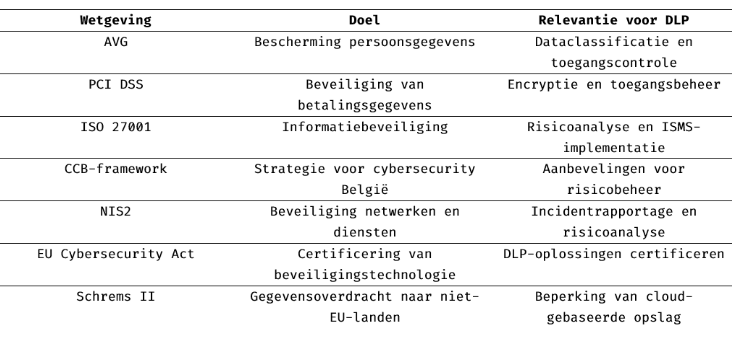
\includegraphics[scale=0.50]
    {img/overzicht.png}
    \caption{\label{fig:overzicht}Overzicht van de belangrijkste wettelijke richtlijnen en uitspraken voor DLP-oplossingen in België.}
  \end{figure}

% Hier beschrijf je de \emph{state-of-the-art} rondom je gekozen onderzoeksdomein, d.w.z.\ een inleidende, doorlopende tekst over het onderzoeksdomein van je bachelorproef. Je steunt daarbij heel sterk op de professionele \emph{vakliteratuur}, en niet zozeer op populariserende teksten voor een breed publiek. Wat is de huidige stand van zaken in dit domein, en wat zijn nog eventuele open vragen (die misschien de aanleiding waren tot je onderzoeksvraag!)?

% Je mag de titel van deze sectie ook aanpassen (literatuurstudie, stand van zaken, enz.). Zijn er al gelijkwaardige onderzoeken gevoerd? Wat concluderen ze? Wat is het verschil met jouw onderzoek?

% Verwijs bij elke introductie van een term of bewering over het domein naar de vakliteratuur, bijvoorbeeld~\autocite{Hykes2013}! Denk zeker goed na welke werken je refereert en waarom.

% Draag zorg voor correcte literatuurverwijzingen! Een bronvermelding hoort thuis \emph{binnen} de zin waar je je op die bron baseert, dus niet er buiten! Maak meteen een verwijzing als je gebruik maakt van een bron. Doe dit dus \emph{niet} aan het einde van een lange paragraaf. Baseer nooit teveel aansluitende tekst op eenzelfde bron.

% Als je informatie over bronnen verzamelt in JabRef, zorg er dan voor dat alle nodige info aanwezig is om de bron terug te vinden (zoals uitvoerig besproken in de lessen Research Methods).

% % Voor literatuurverwijzingen zijn er twee belangrijke commando's:
% % \autocite{KEY} => (Auteur, jaartal) Gebruik dit als de naam van de auteur
% %   geen onderdeel is van de zin.
% % \textcite{KEY} => Auteur (jaartal)  Gebruik dit als de auteursnaam wel een
% %   functie heeft in de zin (bv. ``Uit onderzoek door Doll & Hill (1954) bleek
% %   ...'')

% Je mag deze sectie nog verder onderverdelen in subsecties als dit de structuur van de tekst kan verduidelijken.

%---------- Methodologie ------------------------------------------------------
\section{Methodologie}%
\label{sec:methodologie}

De daadwerkelijke studie naar Data Leakage Prevention (DLP) oplossingen zal theoretisch starten, gevolgd door een praktische Proof of Concept (PoC) in een testomgeving die Evolane zal geven. Hiervoor zal een grondige documentatie opgesteld worden.

\subsection{Omgeving}%

De omgeving zal dienen als testomgeving. Dit zal intern in het bedrijf opgesteld worden. Een licentie van Netskope zal dienen om de DLP-service op te zetten. Deze omgeving zal alle soorten data bevatten (data-in-use, data-in-motion, data-at-rest)  Confidentiële en niet-confidentiële bestanden/data zullen dienen om uit te maken of de DLP-service al het juiste kan identificeren en verdere verwerking kan tegenhouden. De data bestaat vooral uit persoonlijk identificeerbare informatie (PII) en betalingsgegevens (PCI) die verplicht beveiligd moeten zijn door al de opgegeven wetten, richtlijnen of uitspraken (AVG, PCI DSS, ISO 27001, NIS2, Schrems II,..).  Zelf aangemaakte gebruikers met verschillende rechten zullen hierop data doorsturen en verwerken. De testomgeving simuleert realistische klantenscenario’s om te beoordelen hoe effectief deze oplossing werkt.

% \subsection{Regex}%

% !!!!!!!!!!!!!!!!!!!!!!!!!!
% \subsection{Testen}%
% !!!!!!!!!!!!!!!!!!!!!!!!!!

% Hier beschrijf je hoe je van plan bent het onderzoek te voeren. Welke onderzoekstechniek ga je toepassen om elk van je onderzoeksvragen te beantwoorden? Gebruik je hiervoor literatuurstudie, interviews met belanghebbenden (bv.~voor requirements-analyse), experimenten, simulaties, vergelijkende studie, risico-analyse, PoC, \ldots?

% Valt je onderwerp onder één van de typische soorten bachelorproeven die besproken zijn in de lessen Research Methods (bv.\ vergelijkende studie of risico-analyse)? Zorg er dan ook voor dat we duidelijk de verschillende stappen terug vinden die we verwachten in dit soort onderzoek!

% Vermijd onderzoekstechnieken die geen objectieve, meetbare resultaten kunnen opleveren. Enquêtes, bijvoorbeeld, zijn voor een bachelorproef informatica meestal \textbf{niet geschikt}. De antwoorden zijn eerder meningen dan feiten en in de praktijk blijkt het ook bijzonder moeilijk om voldoende respondenten te vinden. Studenten die een enquête willen voeren, hebben meestal ook geen goede definitie van de populatie, waardoor ook niet kan aangetoond worden dat eventuele resultaten representatief zijn.

% Uit dit onderdeel moet duidelijk naar voor komen dat je bachelorproef ook technisch voldoen\-de diepgang zal bevatten. Het zou niet kloppen als een bachelorproef informatica ook door bv.\ een student marketing zou kunnen uitgevoerd worden.

% Je beschrijft ook al welke tools (hardware, software, diensten, \ldots) je denkt hiervoor te gebruiken of te ontwikkelen.

% Probeer ook een tijdschatting te maken. Hoe lang zal je met elke fase van je onderzoek bezig zijn en wat zijn de concrete \emph{deliverables} in elke fase?

%---------- Verwachte resultaten ----------------------------------------------
\section{Verwacht resultaat, conclusie}%
\label{sec:verwachte_resultaten}

Dit onderzoek zal een volledig uitgewerkt Proof of Concept (PoC) opleveren van een Netskope-gebaseerde DLP-oplossing, die is ontworpen om vertrouwelijke gegevens, zoals PII- en PCI-gegevens, te beschermen volgens de Belgische wetgeving. De PoC zal datalekken identificeren en beschermen in een realistische testomgeving die door de klant 'Evolane' mede opgezet zal worden. De vertrouwelijke data zullen in alle mogelijke datatypen voorkomen, zoals data-in-use, data-in-motion en data-at-rest. De oplossing zal gericht zijn op het voorkomen van datalekken die kunnen optreden bij het verwerken en verplaatsen van gevoelige gegevens, zowel binnen als buiten de organisatie.
De proof-of-concept zal een geconfigureerd DLP-platform opleveren dat PII- en PCI-gegevens kan identificeren en beschermen volgens de vooraf ingestelde parameters. Deze parameters zullen voldoen aan klant-specifieke dataclassificaties en zullen worden gevalideerd aan de hand van specifieke testscenario's. Het resultaat van deze tests wordt gepresenteerd in een evaluatierapport, dat de effectiviteit van de oplossing evalueert.
Daarnaast zal het onderzoek aanbevelingen doen over hoe organisaties de Netskope DLP-oplossing kunnen implementeren om te voldoen aan zowel technische als juridische normen. Het verwacht resultaat omvat een succesvolle implementatie van een DLP-oplossing die effectief de risico's van datalekken vermindert.

% Hier beschrijf je welke resultaten je verwacht. Als je metingen en simulaties uitvoert, kan je hier al mock-ups maken van de grafieken samen met de verwachte conclusies. Benoem zeker al je assen en de onderdelen van de grafiek die je gaat gebruiken. Dit zorgt ervoor dat je concreet weet welk soort data je moet verzamelen en hoe je die moet meten.

% Wat heeft de doelgroep van je onderzoek aan het resultaat? Op welke manier zorgt jouw bachelorproef voor een meerwaarde?

% Hier beschrijf je wat je verwacht uit je onderzoek, met de motivatie waarom. Het is \textbf{niet} erg indien uit je onderzoek andere resultaten en conclusies vloeien dan dat je hier beschrijft: het is dan juist interessant om te onderzoeken waarom jouw hypothesen niet overeenkomen met de resultaten.



%%---------- Andere bijlagen --------------------------------------------------
% TODO: Voeg hier eventuele andere bijlagen toe. Bv. als je deze BP voor de
% tweede keer indient, een overzicht van de verbeteringen t.o.v. het origineel.
%\input{...}

%%---------- Backmatter, referentielijst ---------------------------------------

\backmatter{}

\setlength\bibitemsep{2pt} %% Add Some space between the bibliograpy entries
\printbibliography[heading=bibintoc]

\end{document}
